
\chapter{Wprowadzenie}
Dzięki rozwojowi technologii i wzrostowi wydajności sprzętu, gry komputerowe stają się coraz bardziej realistyczne. Dotyczy to nie tylko grafiki, która coraz częściej ma niemal fotograficzną jakość, ale również efektów fizycznych. Prawie każda gra w taki czy inny sposób implementuje prawa rzeczywistego świata. Co więcej, coraz bardziej powszechne staje się wykorzystywanie obliczeń fizycznych zarówno do tworzenia modelu logiki gry, jak~też poprawy jakości wyświetlanej grafiki. Przykładem takiego rozwiązania jest pakiet NVidia VisualFX \cite{bib:nvidia-visualfx}, dostarczający między innymi narzędzia programistyczne do tworzenia realistycznych efektów wizualnych. Jednym z nich jest technologia HairWorks, umożliwiająca generowanie zaawansowanych animacji włosów i sierści reagujących na ruch postaci, wiatr itp. Technologia ta została wykorzystana między innymi w grze Wiedźmin~3: Dziki Gon (rys. \ref{fig:geralt-hairworks}).

\begin{figure}[ht]
	\centering
	\includegraphics[width=0.7\linewidth]{images/geralt-hairworks}
	\caption[Animowane zgodnie z prawami fizyki włosy i~sierść w~grze Wiedźmin~3: Dziki~Gon wykorzystująca technologię NVidia HairWorks]{Animowane zgodnie z prawami fizyki włosy i~sierść w~grze Wiedźmin~3: Dziki~Gon wykorzystująca technologię NVidia HairWorks\newline
		Źródło: \cite{bib:geralt-hairworks}}
	\label{fig:geralt-hairworks}
\end{figure}
\section{Czym jest silnik fizyki?}

Silnik fizyki jest często mylnie traktowany jako tylko moduł do wykrywania kolizji. Istotnie, jest to bardzo ważna, a zarazem często krytyczna (przede wszystkim pod względem wydajności) jego część. W praktyce jednak odpowiedzialność silnika fizycznego jest znacznie większa --- wykonuje on wszystkie obliczenia związane z ruchem, interakcjami i zachowaniem obiektów w~grze. Często również wykonuje dodatkowe, niezwiązane bezpośrednio z mechaniką gry obliczenia, wykorzystywane do udoskonalania animacji i efektów wizualnych. Rysunek \ref{fig:schematsilnika} przedstawia trzy podstawowe funkcjonalności silnika:
\begin{itemize}
	\item ruch obiektów, czyli przykładanie sił oraz rozwiązywanie równań ruchu,
	\item wykrywanie kolizji,
	\item rozwiązywanie kolizji --- aktualizacja parametrów ruchu zgodnie z obliczonymi parametrami odbicia.
\end{itemize}

\begin{figure}[ht]
	\centering
	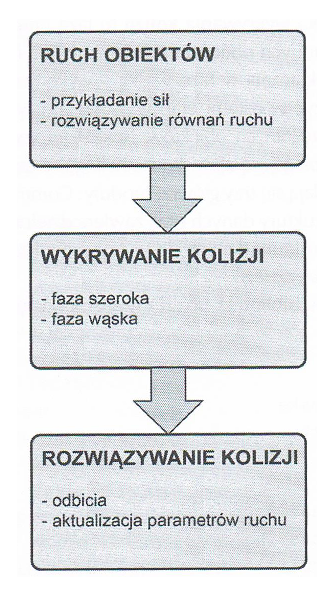
\includegraphics[width=4cm]{images/schemat-silnika.eps}
	\caption[Schemat funkcjonalności silnika fizycznego]{Schemat funkcjonalności silnika fizycznego \newline Źródło: \cite{bib:box2dgrzadka}, strona 35.}
	\label{fig:schematsilnika}
\end{figure}

\section{Rodzaje silników}
Podczas tworzenia silnika fizyki możemy obrać jedno z wielu podejść. Każde z nich charakteryzuje się inną specyfiką działania, różnym stopniem dokładności odwzorowania czy szybkości. Tworząc silnik fizyki dedykowany do gier nie można zapominać o jednym podstawowym założeniu ---  jest to silnik czasu rzeczywistego, co oznacza, że musi on być w stanie działać szybko. Gra powinna być płynna, a obliczenia fizyczne to tylko część całego procesu. Jednocześnie zastosowanie do gier nie wymaga nadzwyczajnej dokładności --- w większości przypadków wystarczy, że zachowanie obiektów jest zbliżone do rzeczywistego. Dzięki temu, że nie ma potrzeby dokładnego odwzorowywania praw fizyki panujących w przyrodzie, można poczynić pewne uproszczenia i optymalizacje, które znacząco przyspieszają działanie modułu. 

Ze względu na zastosowane podejście i różne sposoby modelowania świata, możemy podjąć próbę skategoryzowania silników fizycznych według różnych kryteriów, na przykład \cite{bib:millington}:
\begin{itemize}
	\item \textbf{Sposób modelowania obiektów} --- można wyróżnić silniki oferujące pełne wsparcie dla bryły sztywnej oraz tzw. \textit{mass-aggregate engine}. Takie silniki opisują obiekty za pomocą zbioru połączonych ze sobą wzajemnymi zależnościami punktów materialnych. Implementacja takiego silnika jest prostsza, gdyż nie musi uwzględniać rotacji obiektów, jednak nastręcza wielu problemów.
	\item \textbf{Rozwiązywanie problemu zderzeń} --- obsługa kolizji może zakładać traktowanie każdego zderzenia osobno (metoda iteracyjna). Sposób ten jest szybszy i prostszy w implementacji, ale może prowadzić do niewystarczająco dokładnych wyników w sytuacji, gdy jednocześnie wiele obiektów zderza się ze sobą. Inną metodą jest obliczanie efektów wszystkich zderzeń jednocześnie, z wykorzystaniem macierzy Jacobiego. Sposób ten prowadzi do bardziej realistycznych rezultatów, jednak rozwiązywanie takich układów wielu równań jest niezwykle kosztowne obliczeniowo. 
	\item \textbf{Podejście siłowe i impulsowe}. Ostatnim rozróżnieniem jest sposób, w jaki ciała oddziałują na siebie podczas zderzeń. 
	
	Najprostszym przykładem ilustrującym różnicę między podejściami są kontakty spoczynkowe. Podczas takiego kontaktu siły akcji (siła, z jaką ciało działa np. na podłoże) i reakcji podłoża (wynikająca z III zasady dynamiki Newtona) równoważą się, dzięki czemu ciała pozostają w spoczynku. W~podejściu impulsowym nie stosuje się wprost III zasady dynamiki, takie zachowanie modelowane jest natomiast za pomocą szeregu słabych impulsów generowanych podczas zderzeń. Konsekwencją tego może być, zauważalny przy niewłaściwej konfiguracji, efekt drgania w kontaktach spoczynkowych. Jest on najbardziej widoczny w symulacjach stosów spoczywających na sobie obiektów. 
\end{itemize}

\section{Cel pracy}
W~ramach pracy inżynierskiej \cite{bib:inz} powstał szkielet implementacji, uwzględniający jedynie ruch postępowy oraz zderzenia ciał o~kształcie kolistym. Celem niniejszej pracy było stworzenie na jego podstawie kompletnego, impulsowego silnika fizycznego dedykowanego dla gier 2D implementującego nie tylko dynamikę bryły sztywnej, ale symulującego również ciała miękkie. Problem zderzeń rozwiązywany jest w sposób iteracyjny, natomiast do modelowania obiektów zastosowano podejście mieszane --- zaimplementowano pełne wsparcie dla bryły sztywnej, jednak odkształcenia ciał miękkich modelowane są poprzez agregację masy w cząsteczkach (\textit{mass-aggregate physics}). Dzięki temu uzyskano szybkość obliczeń symulacji bryły sztywnej przy jednoczesnej prostocie modelowania odkształceń obiektów.

\chapter{Część teoretyczna}

\section{Wektory}
\label{part:wektory}
Wektor jest podstawowym pojęciem wykorzystywanym w~opisie ruchu. Poza wartością, wektor posiada punkt przyłożenia, zwrot i~kierunek. W~zapisie matematycznym jest definiowany uporządkowaną parą lub trójką (odpowiednio dla przestrzeni dwu- i~trójwymiarowej) składowych wzdłuż osi układu współrzędnych: 
\[
\vec{v} = (v_x, v_y, v_z),
\]
gdzie $v_x, v_y$ i $v_z$ są składowymi wektora $\vec{v}$ wzdłuż osi OX, OY i OZ. \newline

\subsection{Podstawowe operacje na wektorach}
\subsubsection{Długość wektora}
Definiując wektor $\vec{v}$ jako trójka składowych $(v_x, v_y, v_z)$, możemy obliczyć długość wektora w następujący sposób:
\begin{equation}
|\vec{v}| = \sqrt{v_x^2 + v_y^2 +v_z^2}
\end{equation}

\subsubsection{Wektor przeciwny}
Wektorem przeciwnym nazywamy wektor o tej samej długości i kierunku, ale przeciwnym zwrocie:
\begin{equation}
-\vec{v} = (-v_x, -v_y, -v_z)
\end{equation}
\subsubsection{Normalizacja wektora}
Normalizacją wektora $\vec{v}$ nazywamy taką operację, w wyniku której otrzymujemy wektor jednostkowy (o długości 1) o~takim samym kierunku i~zwrocie co~$\vec{v}$. Możemy go obliczyć w następujący sposób:
\begin{equation}
\hat{v} = \frac{\vec{v}}{ {|\vec{v}|}} = (\frac{v_x} {|\vec{v}|}, \frac{v_y}{|\vec{v}|}, \frac{v_z}{|\vec{v}|})
\end{equation}
\subsubsection{Suma wektorów}
Sumę dwóch wektorów definiujemy jako wektor:
\begin{equation}
\vec{v}+\vec{w} = (v_x+w_x, v_y+w_y, v_z+w_z)
\end{equation}

\subsubsection{Mnożenie wektora przez skalar}
Wynikiem mnożenia wektora $\vec{v}$ przez skalar $a$ jest wektor o kierunku i zwrocie takim samym jak wektor $\vec{v}$, i długości $a$ razy większej od długości tego wektora.
\begin{equation}
a \vec{v} = (a v_x, a v_y, a v_z)
\end{equation}

\subsubsection{Iloczyn skalarny}
\begin{equation}
\vec{v} \circ \vec{w} = v_x w_x + v_y w_y + v_z w_z
\end{equation}
Iloczyn skalarny jest wielkością skalarną. Wartość iloczynu jest równa iloczynowi długości wektorów pomnożoną przez cosinus kąta pomiędzy nimi:
\begin{equation}
\vec{v} \circ \vec{w} = |\vec{v}| |\vec{w}| cos(\alpha)
\end{equation}

\subsubsection{Iloczyn wektorowy} 
Wynikiem iloczynu wektorowego wektora $\vec{v}$ i $\vec{w}$ jest wektor o długości iloczynu długości wektora  $\vec{v}$ i  $\vec{w}$ pomnożony przez sinus kąta pomiędzy  $\vec{v}$ i  $\vec{w}$. \cite{bib:resnick1}. Kierunek wektora wynikowego jest prostopadły do płaszczyzny, na której leżą wektory, natomiast zwrot można wyznaczyć z reguły prawej dłoni \footnote{Reguła ta jest opisana szczegółowo w \cite{bib:resnick1}, Rozdział 3.7, str. 50, natomiast z punktu widzenia obliczeń przeprowadzanych za pomocą komputera znacznie bardziej użyteczny jest wzór \ref{eq:vectorcross}.}. 
Iloczyn wektorowy może być również obliczony z wykorzystaniem składowych w następujący sposób:
\begin{equation}
\vec{v} \times \vec{w} = (v_y w_z - w_y v_z, v_z w_x - w_z v_x, v_x w_y-w_x v_y)
\label{eq:vectorcross}
\end{equation}

\section{Przekształcenia geometryczne}
\label{part:macierze}
Macierze są wygodnym i szybkim sposobem zapisu przekształceń geometrycznych, pozwalającym na wydajne ich nakładanie na punkty przestrzeni. Dzięki temu zapis macierzowy jest obecnie najpopularniejszym sposobem zapisu przekształceń wykorzystywanym w grafice komputerowej. \cite{bib:smurf-geometria}. 

\subsection{Współrzędne jednorodne}
\label{part:wspolrzednejednorodne}
Niech $ P_k = (x_p, y_p) $ opisuje punkt w dwuwymiarowej przestrzeni kartezjańskiej. Wówczas współrzędne jednorodne znormalizowane dla tego punktu przyjmują postać $ P = (x_p, y_p, 1) $. Dzięki zastosowaniu współrzędnych jednorodnych przekształcenia geometryczne możemy zapisać w prosty sposób --- za pomocą odpowiedniego mnożenia macierzy. 

Dla macierzy $M$ o wymiarach 3x3 będącej zapisem przekształcenia geometrycznego, transformację punktu $P$ reprezentuje operacja mnożenia:

\begin{equation}
P'^T = M \cdot P^T,
\end{equation}
gdzie $P'$ jest wektorem $P' = (x'_p,y'_p, 1)$ opisującym położenie punktu $P$ po transformacji.

\subsection{Tożsamość}
Przekształcenie tożsamościowe jest reprezentowane przez macierz jednostkową $I$:
\begin{equation}
I = \left[ \begin{array}{ccc}
1 & 0 & 0 \\
0 & 1 & 0 \\
0 & 0 & 1
\end{array} \right]
\label{eq:macierz-jedn}
\end{equation}

\subsection{Obrót}
Operacje obrotu wokół początku układu współrzędnych o kąt $\phi$ opisuje macierz $M_O$:
\begin{equation}
M_O = \left[ \begin{array}{ccc}
cos(\phi) & -sin(\phi) & 0 \\
sin(\phi) & cos(\phi) & 0 \\
0 & 0 & 1
\end{array} \right]
\label{eq:macierz-obrot}
\end{equation}

\subsection{Translacja}
Przesunięcie o wektor $T = (x_t, y_t) $ opisuje macierz $M_T$:
\begin{equation}
M_T = \left[ \begin{array}{ccc}
1 & 0 & x_t \\
0 & 1 & y_t \\
0 & 0 & 1
\end{array} \right]
\label{eq:macierz-translacja}
\end{equation}

\subsection{Skalowanie}
Przekształcenie skalowania można opisać za pomocą macierzy $M_S$ postaci:
\begin{equation}
M_O = \left[ \begin{array}{ccc}
s_x & 0 & 0 \\
0 & s_y & 0 \\
0 & 0 & 1
\end{array} \right], 
\label{eq:macierz-skalowanie}
\end{equation}
gdzie $s_x$ jest współczynnikiem skali względem osi $OX$, natomiast $s_y$ - względem osi $OY$. 

\subsection{Złożenie przekształceń}
Dla dowolnych transformacji geometrycznych opisanych macierzami $M_1$ i $M_2$, macierz $M_C = M_2 \cdot M_1 $ opisuje przekształcenie będące wynikiem złożenia transformacji $M_1$ i $M_2$. Złożenie przekształceń pozwala na szybsze i wydajniejsze realizowanie transformacji --- zamiast wykonywać $n$ operacji mnożenia macierzy przez wektor, można zastosować pojedyncze mnożenie wektora przez macierz będącą złożeniem wszystkich przekształceń.
\label{part:zlozenie-przeksztalcen}

\section{Zasady dynamiki Newtona}
\label{part:zasadynewtona}
Isaac Newton w swojej pracy \textit{Philosophiae Naturalis Principia Mathematica} opublikowanej w 1687 roku sformułował trzy podstawowe zasady dynamiki. Są one fundamentem mechaniki klasycznej, a zatem stanowią podstawę i punkt wyjścia podczas modelowania ruchu obiektów.

\subsection{I zasada dynamiki Newtona}
\begin{quote}
	,,Jeśli wypadkowa sił działających na ciało jest równa zeru $\vec{(F_{wyp}} = 0)$, to nie może zmienić się jego prędkość, czyli nie może ono przyspieszyć.\newline
	Innymi słowy, jeśli ciało spoczywa, to pozostanie w spoczynku, a jeśli się porusza, to będzie się nadal poruszać z tą samą prędkością (to znaczy z prędkością o tej samej wartości i kierunku).''\newline
	\cite[Strona 88, rozdział 5.2]{bib:resnick1}
\end{quote}

Zasada ta jest szczególnym przypadkiem drugiej zasady dynamiki, i wynika również z równania \ref{eq:newt2} --- jeżeli na ciało nie działa żadna siła ($\vec{F_{wyp}} = 0$), to przyspieszenie jest równe zero. 

\subsection{II zasada dynamiki Newtona}
\label{part:drugazasadanewtona}
\begin{quote}
	,,Siła wypadkowa działająca na ciało jest równa iloczynowi masy tego ciała i jego przyspieszenia.'' \newline
	\cite[Strona 91, rozdział 5.5]{bib:resnick1} 
\end{quote}
II zasadę dynamiki możemy zapisać również jako równanie 
\begin{equation}
\vec{F_{wyp}}=m\vec{a}
\label{eq:newt2},
\end{equation}
w~którym $\vec{F_{wyp}}$ oznacza wypadkową wszystkich sił działających na~dane ciało, $m$~-~masę ciała, natomiast $\vec{a}$ - przyspieszenie ciała.

\subsection{III zasada dynamiki Newtona}
\begin{quote}
	,,Gdy dwa ciała oddziałują ze sobą, siły, jakimi działają one na siebie mają taką samą wartość bezwzględną i przeciwne kierunki.'' \newline
	\cite[strona 100, rozdział 5.7]{bib:resnick1}
\end{quote} 
Zasada ta mówi, że jeśli ciało działa na inne ciało siłą, to drugie ciało działa na pierwsze siłą przeciwną (mającą taką samą wartość, lecz przeciwny zwrot). Podczas implementacji silnika fizyki zasada jest o tyle istotna, że należy pamiętać o tym, aby wszystkie siły wewnętrzne (generowane przez silnik, na przykład wskutek zderzeń) były jednocześnie przykładane do obu ciał.

\section{Zasada zachowania pędu}
\label{part:zachowaniapedu}
\begin{quotation}
	,,Jeżeli na układ cząstek nie działają siły zewnętrzne lub ich wypadkowa jest równa zeru, to całkowity pęd $\vec{p}$ układu nie ulega zmianie.''\newline
	\cite[Strona 216, rozdział 9.6]{bib:resnick1}
\end{quotation}

Pęd jest wielkością wektorową zdefiniowaną następująco:
\begin{equation}
\vec{p} = m\vec{v},
\end{equation}
gdzie $m$ oznacza masę ciała, natomiast $\vec{v}$ --- jego prędkość.

Prawo to ma szczególne zastosowanie podczas zderzeń ciał --- wtedy korzystając z niego możemy obliczyć ich prędkości po zderzeniu nie znając sił, jakie oddziałują pomiędzy ciałami w trakcie zderzenia.
Prawo to jest niezwykle przydatne podczas rozwiązywania problemu kolizji i~określania stanu obiektów po zderzeniu. Dzięki jego wykorzystaniu nie ma potrzeby określania sił działających podczas zderzeń, a~jedynie określenie stanu obiektu po zderzeniu na podstawie jego parametrów.
\section{Ruch obrotowy}
\subsection{Zasady dynamiki ruchu obrotowego}
\label{part:zasadydynamikiobr}
W ruchu obrotowym analogiczną wartością do siły dla ruchu postępowego jest moment siły. Moment siły definiujemy jako iloczyn wektorowy ramienia siły oraz wektora siły:
\begin{equation}
\label{eq:moment-sily}
\vec{\tau} = \vec{r} \times \vec{F}.
\end{equation}
Ramieniem siły $\vec{r}$ nazywamy wektor o początku w osi obrotu ciała, a końcu w punkcie przyłożenia siły. 

Wielkością analogiczną do pędu w ruchu postępowym, w ruchu obrotowym jest moment pędu $L$ definiowanym jako:
\begin{equation}
\label{eq:moment-pedu}
\vec{L} = \vec{r} \times \vec{p},
\end{equation}
gdzie $\vec{p}$ jest pędem ciała.
Zasady dynamiki dla ruchu obrotowego są analogiczne do tych sformułowanych w XVIIw. przez Newtona dla ruchu postępowego:
\begin{quotation}
	\textbf{I zasada dynamiki dla ruchu obrotowego}\\
	,,Ciało sztywne, na które nie działa moment siły pozostaje w spoczynku lub porusza się ruchem obrotowym jednostajnym.'' \\	
	Źródło: \cite{bib:kakol}
\end{quotation}

\begin{quotation}
	\textbf{II zasada dynamiki dla ruchu obrotowego} \\
	,,Wypadkowy moment siły działający na punkt materialny jest równy prędkości zmian momentu pędu.''\\
	Źródło: \cite{bib:kakol}
\end{quotation}
Drugą zasadę dynamiki można również zapisać w postaci równania
\begin{equation}
\vec{L} = I \cdot \vec{\tau},
\end{equation}
gdzie $I$ jest wielkością charakteryzującą dane ciało, zwaną momentem bezwładności.

\begin{quotation}
	\textbf{III zasada dynamiki dla ruchu obrotowego}\\
	,,Jeżeli dwa ciała oddziałują wzajemnie, to moment sił z jakim działa ciało drugie na ciało pierwsze jest równy i przeciwnie skierowany do momentu siły, z jakim ciało pierwsze działa na drugie.''\\
	Źródło: \cite{bib:kakol}
\end{quotation}

Zasady dynamiki dla ruchu obrotowego są analogiczne jak te zdefiniowane przez Newtona dla ruchu postępowego --- jedynymi różnicami są rodzaj ruchu. Prędkość, przyspieszenie oraz siła  są zamieniane na wielkości analogiczne dla ruchu obrotowego --- prędkość, przyspieszenie obrotowe i moment siły. Analogiem dla masy w ruchu obrotowym jest moment bezwładności. 

\subsection{Moment bezwładności}
Moment bezwładności określa moment siły jaki trzeba przyłożyć do ciała, aby uzyskać określoną zmianę prędkości kątowej. Moment bezwładności jest określany względem danej osi obrotu i definiowany jest jako:
\begin{equation}
\label{eq:moment-bezwladnosci}
I = \int r^2 dm
\end{equation}

\subsubsection*{Twierdzenie Steinera}
\label{part:twsteinera}
Dzięki twierdzeniu Steinera możemy w prosty sposób wyliczyć moment bezwładności danego ciała względem dowolnej osi obrotu. Dzięki temu można raz obliczony moment bezwładności dla osi względem środka masy ciała wykorzystać do obliczenia momentu wokół innej osi (w~przypadku silnika fizycznego --- w~szczególności w~punkcie zderzenia ciał).
Twierdzenie Steinera wyrażone jest wzorem:
\begin{equation}
I = I_0 + md^2,
\end{equation}
gdzie $I_0$ --- moment bezwładności względem osi obrotu przechodzącej przez środek masy, $m$ --- masa ciała, natomiast $d$ --- przesunięcie (odległość) względem osi bazowej.
%\section{* Siła sprężystości}
%\improvement{Siła sprężystości?}
%\section{Siła sprężystości}
%\label{part:silasprezystosci}
%Siła sprężystości jest to siła działająca po odkształceniu ciała sprawiająca, że ciało powraca do swojego pierwotnego kształtu. Dla małych odkształceń siła ta jest wprost proporcjonalna do odkształcenia.
%\begin{quote}
%	,,naprężenie i odkształcenie są do siebie proporcjonalne (...). Odpowiedni współczynnik proporcjonalności nazywa się modułem sprężystości, tak że
%	\begin{equation}
%	\text{naprężenie} = \text{(moduł sprężystości)} \cdot \text{(odkształcenie)}.''
%	\label{eq:hooke}
%	\end{equation} \newline
%	\cite[strona 15, rozdział 13.6]{bib:resnick2}
%\end{quote} 
%\subsection{Oscylator harmoniczny}
%Ciało na które działa siła sprężystości, np. ciało przymocowane do sprężyny, mogące swobodnie się poruszać 

\chapter{Implementacja}
\label{cha:implementacja}
Silnik fizyki został napisany w języku C\# dla platformy .Net Framework. Jest to środowisko uruchomieniowe aplikacji rozwijane przez firmę Microsoft od 2002 roku. Część założeń platformy, takich jak automatyczne zarządzanie pamięcią i czasem życia obiektów, kompilacja do kodu pośredniego (CIL/\textit{bytecode}) oraz JIT (\textit{Just In Time Compilation}), czy wsparcie dla wielu języków programowania, jest podobnych do środowiska JVM (maszyna wirtualna Javy) \cite{bib:msdndotnet}. Język ten od wielu lat zyskuje również popularność wśród programistów gier, dzięki powstawaniu wielu bibliotek i silników do ich tworzenia. Jednym z pierwszych był rozwijany w celu spopularyzowania i zwiększenia ilości gier na Xboksa 360 zestaw bibliotek Microsoft XNA, udostępniający poza wspominaną plarformą Xbox 360 możliwość pisania gier również na systemy operacyjne Windows oraz Windows Phone \cite{bib:cotojestxna}. Ogromny wpływ na popularyzację C\# jako języka do pisania gier miało powstanie Unity3D. Jest to obecnie najczęściej wykorzystywany silnik do tworzenia gier, w szczególności mobilnych --- 34\% gier spośród tysiąca najpopularniejszych na platformy mobilne zostało stworzonych za pomocą Unity (dane za I kwartał 2016) \cite{bib:popularnosc-unity}. 

\section{Biblioteka przekształceń i operacji geometrycznych}
W ramach pracy zaimplementowano klasy \verb|Vector2| i~\verb|Matrix3| wspierające rachunek wektorowy oraz zbiór kilku algorytmów wykorzystywanych do symulacji. Nie mają one bezpośredniego związku z fizyką i nie stanowią implementacji samego silnika fizycznego, dlatego zostały wyodrębnione do osobnego podprojektu i~stanowią swoistą bibliotekę do manipulacji obiektami geometrycznymi, zaimportowaną i wykorzystywaną w~implementacji silnika. Biblioteka ta składa się z następujących elementów:

\subsection{Rachunek wektorowy}
Przestrzeń nazw \verb|Geometry.Vector| zawiera definicje dwu- i~trójwymiarowego wektora. Klasy \verb|Vector2| i \verb|Vector3| posiadają przeładowane operatory (dodawania, odejmowania oraz mnożenia przez wektor i skalar oraz jednoargumentowy \verb|-|), umożliwiające czytelny i intuicyjny zapis operacji. Z~racji tego, że \verb|Vector3| jest wykorzystywany głównie do wyrażania dwuwymiarowej wielkości we współrzędnych jednorodnych, zdefiniowano również operator konwersji wektora trójwymiarowego do dwuwymiarowego (obcinający ostatnią współrzędną), oraz metodę \verb|.AsVector3()|, konwertujący dwuwymiarowy wektor do współrzędnych jednorodnych.

Dzięki wykorzystaniu funkcjonalności najnowszej, siódmej wersji języka C\# (oficjalna premiera miała miejsce wraz z~premierą środowiska Visual Studio 2017 7 marca 2017 \cite{bib:visual2k17releasenotes}) --- nowej składni użycia klasy \verb|Tuple| \cite{bib:whatsnewin7}, oraz przeładowaniu operatora niejawnej konwersji, operacje na wektorach są jeszcze prostsze i bardziej intuicyjne --- przypominają naturalny zapis matematyczny. Implementację mechanizmu i przykład wykorzystania ilustrują listingi \ref{lst:vector2implicitconversion} oraz \ref{lst:vector2manipulation}.

\lstinputlisting[label={lst:vector2implicitconversion}, caption={Definicja operatora niejawnej konwersji typu \texttt{Tuple} do wektora}, firstline=71,lastline=74]{../Geometry/Vector/Vector2.cs}

\lstinputlisting[label={lst:vector2manipulation}, caption={Przykład użycia operatora niejawnej konwersji jako test z~wykorzystaniem frameworka NUnit}, firstline=14,lastline=21]{../GeometryTests/VectorShowcase.cs}

\subsection{Definicje obiektów geometrycznych}
Przestrzeń nazw \verb|Geometry.Shapes| zawiera definicje podstawowych obiektów geometrycznych: prostej (\verb|Line|), odcinka (\verb|Segment|), okręgu (\verb|Circle|) i wielokąta (\verb|Polygon|) wraz z~metodami umożliwiającymi proste ich tworzenie i~podstawowe operacje przekształceń. Dla wielokąta na przykład stworzono statyczne funkcje fabrykujące (ang. \textit{factory method}) \verb|AARectangle|, pozwalającą na stworzenie prostokąta o bokach równoległych do osi układu współrzędnych (ang. \textit{Axis-aligned rectangle}), \verb|RegularPolygon|, tworzącą wielokąt foremny o zadanej liczbie wierzchołków, oraz \verb|RandomPolygon|, pozwalającą na stworzenie losowego nieforemnego wielotąta.

Dla prostej, w celu znacznego ułatwienia operacji z nimi związanych, poza możliwością zdefiniowana jej na kilka sposobów: bezpośrednio z podaniem parametrów \texttt{a} i \texttt{b}, z odcinka, dwóch punktów czy poprzez podanie kierunku i punktu, przez który ma przechodzić, zdefiniowano również szereg metod pomocniczych (przedstawionych na listingu \ref{lst:lineutils}), umożliwiających:
\begin{itemize}
	\item obliczenie odległości punktu od prostej,
	\item znalezienia przecięcia dwóch prostych,
	\item wykreślenia prostopadłej lub równoległej do zadanej, przechodzącej przez punkt.
\end{itemize}

\lstinputlisting[label={lst:lineutils}, caption={Metody umożliwiające przekształcenia i~obliczenia na prostych}]{../Geometry/Shapes/LineUtils.cs}

\subsection{Przekształcenia macierzowe}
Klasa macierzy 3x3, implementująca opisane w podrozdziale \ref{part:macierze} przekształcenia geometryczne w dwuwymiarowym układzie współrzędnych, została zdefiniowana w~przestrzeni nazw \verb|Geometry.Matrix|. Klasa ta, dzięki szeregowi metod fabrykujących oraz przeładowaniu \mbox{operatora} mnożenia, dostarcza intuicyjny mechanizm pozwalający na łatwe definiowanie przekształceń. 

Pomimo, że taka operacja z matematycznego punktu widzenia jest niemożliwa, zdefiniowano również operator mnożenia macierzy 3x3 przez dwuwymiarowy wektor (listing \ref{lst:matrixvectormultiplication}). Operacja ta zwraca mnożony wektor z nałożonym przekształceniem wyrażanym przez macierz. Matematycznie odpowiada to mnożeniu macierzy przez transponowany wektor skonwertowany do współrzędnych jednorodnych, jednak niejawne wykonywanie tych operacji pozwala uczynić zapis bardziej zwięzłym i czytelnym, oraz umożliwia przechowywanie współrzędnych w~bardziej intuicyjnej, a~także oszczędnej pamięciowo formie --- bez przechowywania nadmiarowej trzeciej współrzędnej.

\lstinputlisting[label={lst:matrixvectormultiplication}, caption={Operator mnożenia macierzy \texttt{Matrix3} przez \texttt{Vector2} --- aplikacja przekształcenia geometrycznego}, firstline=97,lastline=104]{../Geometry/Matrix/Matrix3.cs}

\subsection{Pozostałe algorytmy}
Oprócz rachunku wektorowego i macierzowego, a także klas reprezentujących obiekty geometryczne, biblioteka \verb|Geometry| zawiera również kilka algorytmów użytecznych z punktu widzenia silnika fizycznego.

\subsubsection{Pole powierzchni wielokąta}
Algorytm obliczania pola powierzchni wielokąta opiera się o~wzory Gaussa, zwane również \textit{shoelace formula}. Pole wielokąta można obliczyć w~następujący sposób \cite{bib:geodezja1}:
\begin{equation}
2P = \sum_{1}^{n}{x_{i+1}-x_{i-1}y_i}.
\end{equation}
Implementacja algorytmu przedstawiona jest na listingu \ref{lst:areacalculator}.

\clearpage
\lstinputlisting[label={lst:areacalculator}, caption={Implementacja algorytmu obliczającego pole powierzchni wielokąta}, firstline=21, lastline=34]{../Geometry/AreaCalculator.cs}

\subsubsection{Triangulacja}
\label{part:triangulacja}
Triangulacja wielokąta jest procesem podziału wielokąta prostego (rys. \ref{fig:triangulacja-wielokatprosty}) na nienakładające się trójkąty tak, że wszystkie wierzchołki otrzymanych trójkątów są jednocześnie wierzchołkami wielokąta. W~tym celu wykorzystano algorytm ,,obcinania uszu'' (ang. \textit{ear clipping}) \cite{bib:eberlytriangulation}. Algorytm ten jest najprostszym algorytmem triangulacji, o~asymptotycznej złożoności obliczeniowej rzędu $O(n^2)$. Algorytmy o~niższej złożoności, rzędu $O(n \log n)$ co prawda istnieją, ale są zdecydowanie bardziej złożone w~implementacji. W~praktyce jednak algorytm jest uruchamiany dla wielokątów o~stosunkowo niewielkiej liczbie wierzchołków.
\begin{figure}[ht]
	\centering
	\includegraphics[width=0.8\linewidth]{images/triangulacja-wielokatprosty}
	\caption[Przykład wielokąta prostego]{Na powyższym rysunku jedynie wielokąt 1. jest wielokątem prostym --- każdy wierzchołek należy do dokładnie dwóch krawędzi, oraz odcinki przecinają się tylko w~wierzchołkach. Źródło: \cite{bib:eberlytriangulation}}
	\label{fig:triangulacja-wielokatprosty}
\end{figure}

Algorytm obcinania uszu opiera się na wykrywaniu i~usuwaniu z wielokąta tzw. uszu --- takich trójkątów złożonych z~trzech kolejnych wierzchołków wielokąta, że:
\begin{itemize}
	\item dwa boki trójkąta są równocześnie bokami wielokąta,
	\item trzeci bok trójkąta jest przekątną wielokąta zawierającą się w całości we wnętrzu figury,
	\item trójkąt nie zawiera innych wierzchołków wielokąta niż wierzchołki trójkąta.
\end{itemize}

\begin{figure}[ht]
	\centering
	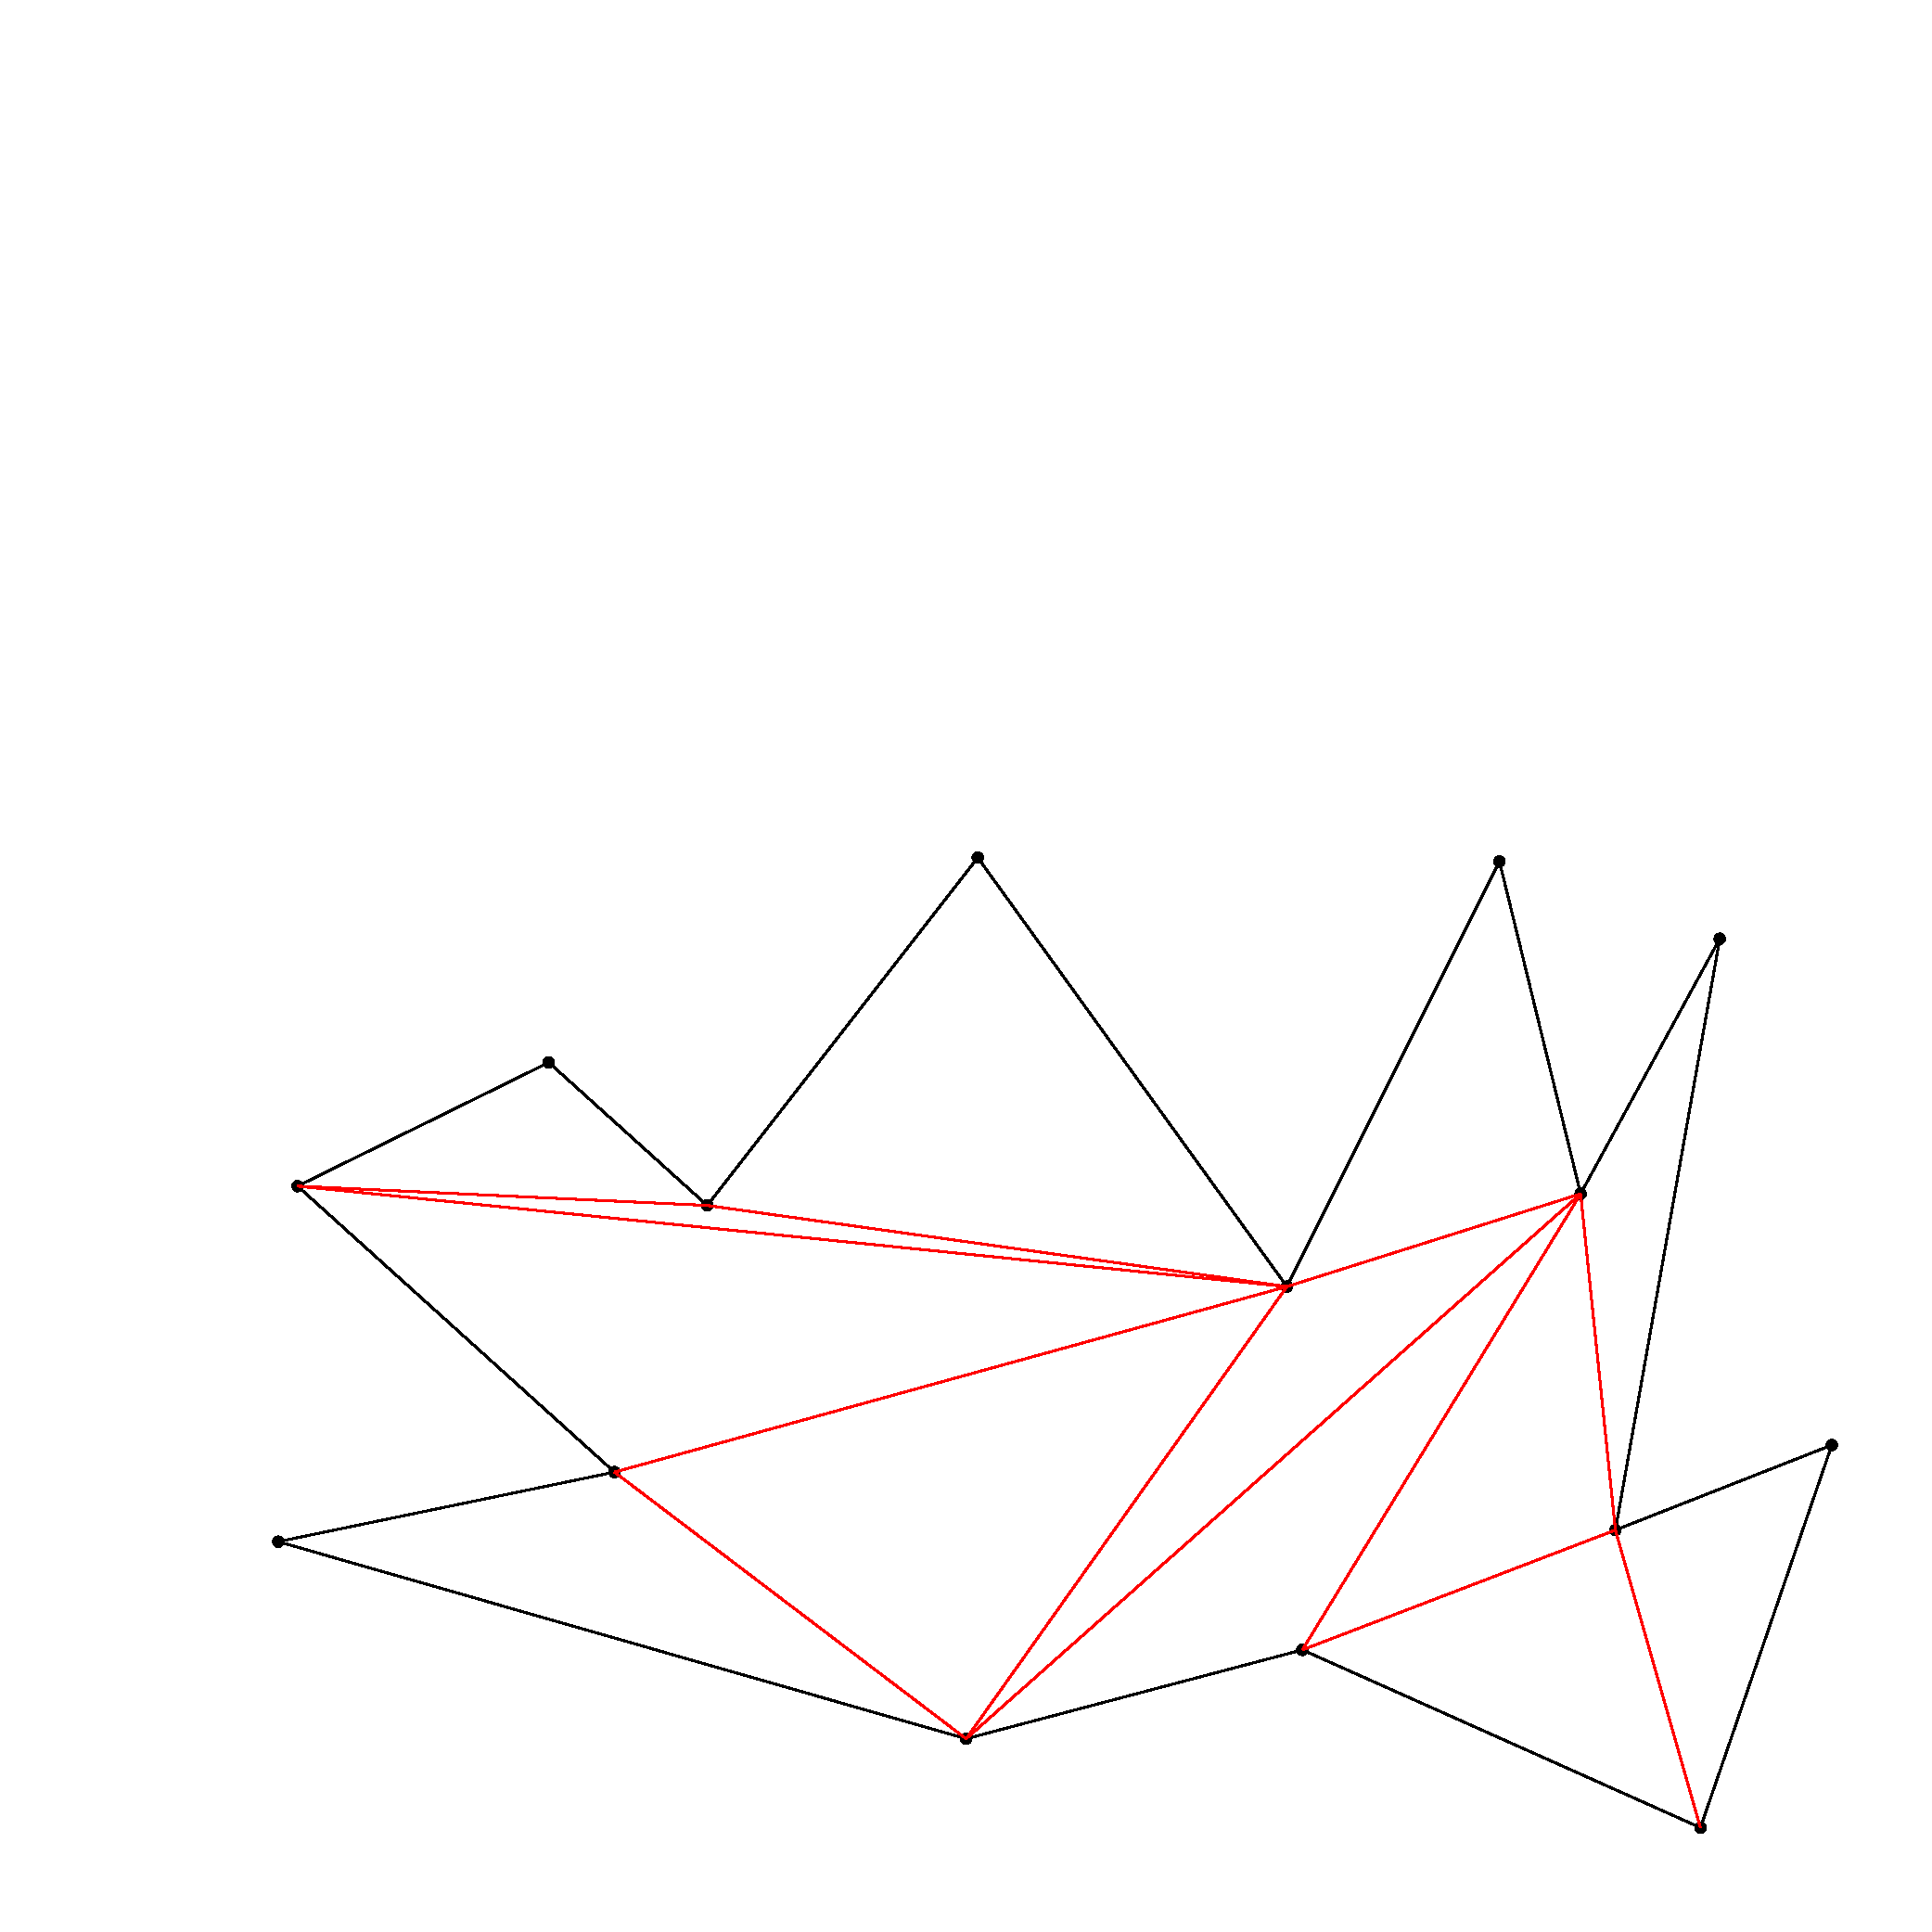
\includegraphics[width=0.7\linewidth]{images/triangulacja-przyklad}
	\includegraphics[width=0.3\linewidth]{images/triangulacja-prostokat}
	\caption[Przykładowy podział wklęsłego wielokąta oraz prostokąta z punktami pośrednimi na trójkąty z wykorzystaniem algorytmu obcinania uszu]{Przykładowy podział wklęsłego wielokąta oraz prostokąta z punktami pośrednimi na trójkąty z wykorzystaniem algorytmu obcinania uszu. \newline Źródło: opracowanie własne}
	\label{fig:triangulacja-przyklad}
\end{figure}

Triangulacja polega na sekwencyjnym znajdowaniu kolejnych uszu i~ich usuwaniu. Każda taka operacja redukuje o~1~ilość pozostałych wierzchołków. Proces jest powtarzany, dopóki nie pozostanie pojedynczy trójkąt. W~ten sposób początkowa figura zawierająca n~wierzchołków dzielona jest na n-2~trójkątów. Przykładowy podział wielokąta na trójkąty przedstawiony jest na rysunku \ref{fig:triangulacja-przyklad}.

\subsubsection{Całkowanie po powierzchni wielokąta}
\label{part:calkapowielokacie}
Algorytm całkowania numerycznego po powierzchni dowolnego wielokąta wypukłego przybliża całkowaną figurę szeregiem trójkątów o wierzchołkach:
\begin{itemize}
	\item w~obranym punkcie $S$ leżącym wewnątrz całkowanej figury (,,środka całkowania''), oraz
	\item punktach $E$ i $F$ leżących na krawędzi wielokąta tak, że ramiona $b_1$ i~$b_2$~tworzą kąt o~mierze $d\phi$, będącej krokiem całkowania (rys. \ref{fig:calkowanie-trojkaty}).
\end{itemize}

\begin{figure}[ht]
	\centering
	\includegraphics[width=0.7\linewidth]{images/calkowanie-trojkaty}
	\caption[Schemat podziału całkowanej figury]{Schemat podziału całkowanej figury\newline Źródło: oprac. własne}
	\label{fig:calkowanie-trojkaty}
\end{figure}

Ponieważ $d\phi \rightarrow 0$, $b_1 \approx b_2 \approx h$. Trójkąt ten może zatem być przybliżony trójkątem równoramiennym o wysokości $h$ i podstawie $a=h \tan{d\phi}$. Kąt $d\phi$ oraz wysokość są przekazywane jako parametry wywołania funkcji całkującej, przybliżającej wartość całki dla danego fragmentu figury.

W praktyce działanie algorytmu sprowadza się do obliczenia długości kolejnych odcinków $SI$ wyznaczonych jako przecięcie promieni wyprowadzonych z punktu $S$ co kąt $d\phi$ oraz sumowaniu rezultatu wywołania dla każdego z~nich dwuparametrowej funkcji całkującej. Kod implementujący powyższy algorytm przedstawiony jest na listingu \ref{lst:integral}.	Poprawność algorytmu została przetestowana testami jednostkowymi obliczającymi pole powierzchni wielokąta (listing \ref{lst:integraltests}).

\lstinputlisting[label={lst:integral}, caption={Implementacja algorytmu całkowania po powierzchni dowolnego wielokąta wypukłego}, firstline=10,lastline=36]{../Geometry/PolygonIntegral.cs}

\lstinputlisting[label={lst:integraltests}, caption={Testy algorytmu całkowania numerycznego }, firstline=31,lastline=46]{../GeometryTests/PolygonIntegralTests.cs}

\subsubsection{Geometryczny moment bezwładności}
\label{part:momentbezwladnosci}
Moment bezwładności ciała względem dowolnej osi obrotu jest zdefiniowany jako wartość następującej całki po powierzchni (lub dla trzech wymiarów objętości) ciała \cite{bib:kakol-wyklad}:
\begin{equation}
\int_{P}^{} r^2 dm,
\end{equation}
gdzie $r$ jest odległością od osi obrotu. 
Geometrycznym momentem bezwładności nazywany jest moment bezwładności jednorodnej bryły podzielony przez jego gęstość, obliczany jako wartość całki \cite{bib:wiki-geombezwl}:
\begin{equation}
I_G = \int_{V}^{} r^2 dV.
\end{equation} 
Może zostać łatwo wykorzystany do obliczenia momentu bezwładności ciała o~stałej gęstości względem środka masy:
\begin{equation}
I = \rho \cdot I_G.
\end{equation}

Algorytm obliczający geometryczny moment bezwładności dowolnego wielokąta wypukłego przedstawiony jest na listingu \ref{lst:moment}. Wykorzystuje on funkcję całkującą po powierzchni wielokąta (\ref{part:calkapowielokacie}) i~działa według schematu:
\begin{enumerate}
	\item \label {pt:srodekmasy1} Podziel figurę na trójkąty wykorzystując algorytm triangulacji (\ref{part:triangulacja}),
	\item Dla każdego trójkąta: 
	\begin{enumerate}
		\item wyznacz długości boków $a, b, c$
		\item oblicz pole powierzchni tego trójkąta,
		\item wyznacz środek masy jako punkt przecięcia środkowych boków,
	\end{enumerate}
	\item \label{pt:srodekmasy} oblicz środek masy figury jako średnia ważona środków masy poszczególnych trójkątów z~wagami równymi polu ich powierzchni,
	\item oblicz geometryczny moment bezwładności figury z~wykorzystaniem algorytmu całkowania numerycznego:
	\begin{enumerate}
		\item punktem środkowym całkowania jest środek masy figury, obliczony w pkt.~\ref{pt:srodekmasy1}-\ref{pt:srodekmasy},
		\item Funkcja przybliżająca moment bezwładności dla trójkąta równoramiennego (podstawowego wycinka figury podczas całkowania) --- według wzoru \ref{eq:moment-trojkata-final}.
		\begin{equation}
		\label{eq:moment-trojkata-final}
		I(d\phi, h) = \frac{1}{4} h^4 \cdot d\phi.
		\end{equation}
		Wzór ten został wyznaczony empirycznie. Moment bezwładności dla figury płaskiej ma wymiar długość$^4$, zatem wyjściowy wzór na moment bezwładności trójkąta:
		\begin{equation}
		I(d\phi, h) = x \cdot h^4 \tan(\frac{d\phi}{2}),
		\end{equation}
		gdzie $x$ --- brakujący współczynnik, $h$ --- wysokość trójkąta, $d\phi$ --- miara kąta wierzchołkowego przy wierzchołku będącym środkiem całkowania figury.
		
		Ponieważ $d\phi \Rightarrow 0$, $tan\alpha \approx \alpha$. Zatem wzór można uprościć następującym przybliżeniem:
		\begin{equation}
				I(d\phi, h) = x \cdot h^4 \frac{d\phi}{2}.
		\end{equation}
		Po napisaniu testów z~kilkoma przypadkami testowymi wyznaczono wartość $x$ na $\frac{1}{2}$, co w~ostateczności daje przybliżony wzór  \ref{eq:moment-trojkata-final}.
	\end{enumerate}
\end{enumerate}
\clearpage
\lstinputlisting[label={lst:moment}, caption={Funkcja obliczająca geometryczny moment bezwładności dowolnego wielokąta wypukłego}, firstline=36, lastline=77]{../Geometry/InertiaCalculator.cs}
\lstinputlisting[label={lst:testy-momentu}, caption={Testy obliczeń momentu bezwładności wielokąta},firstline=10, lastline=53]{../GeometryTests/InertiaCalculatorTests.cs}

\section{Struktura silnika}

Rysunek \ref{fig:schemat-silnika-vs} przedstawia uproszczoną strukturę kodu zaimplementowanego silnika fizycznego. Odzwierciedla ona w pewnym stopniu schemat funkcjonalności (rys. \ref{fig:schematsilnika}) --- submoduł \verb|Physics.Bodies| zawiera definicje klas reprezentujących symulowane obiekty, które wraz z \verb|Physics.Force| są odpowiedzialne za przykładanie sił i aktualizację parametrów obiektów. \verb|Physics.Collision.Detection| odpowiada za wykrywanie zderzeń, natomiast \verb|Physics.Collision.Handling| --- reakcję na nią. Dodatkowo przestrzeń nazw \verb|Physics.Constraints| zawiera klasy odpowiedzialne za realizację złączeń obiektów. Większość modułu korzysta z podprojektu \verb|Geometry|, w którym zaimplementowano rachunek wektorowy, przekształcenia geometryczne oraz algorytmy --- triangulacji, obliczania pola powierzchni figury, całkowania po powierzchni wielokąta oraz obliczania geometrycznego momentu bezwładności.
\begin{figure}[htb]
	\centering
	\includegraphics[width=\linewidth]{images/schemat-silnika-vs}
	\caption{Struktura projektu stworzonego silnika fizycznego. \newline
		Źródło: opracowanie własne
		% todo prawdopodobnie z BODY wyciągnie się rigidbody i softbody, wrzucic aktualne na koncu
	}
	\label{fig:schemat-silnika-vs}
\end{figure}

\section{Bryła sztywna}
Klasa \verb|RigidBody| reprezentuje bryłę sztywną oraz implementuje logikę związaną z jej symulacją. Obiekt \verb|RigidBody| posiada właściwości opisujące dane ciało, takie jak masę, kształt czy materiał oraz stan, w jakim się znajduje --- położenie, rotację, prędkość itd. Odpowiedzialnością tej klasy jest aktualizacja stanu w kolejnych krokach czasowych. Realizuje to metoda \verb|Update| (listing \ref{lst:rigidbody-update}).

\subsection{Impulsy}
Impuls, zwany również popędem siły jest iloczynem wektora siły i czasu jej działania \cite{bib:wiki-impuls}. Impuls do ciała jest przykładany poprzez wywołanie metody \verb|ApplyImpulse|, wymagającej dwóch parametrów: wartości impulsu oraz wektora ramienia siły (czyli punktu przyłożenia we współrzędnych lokalnych ciała). Metodę aplikującą impuls, będącą jednocześnie wyrażeniem II zasady dynamiki Newtona dla ruchu postępowego i~obrotowego (zob. \ref{part:drugazasadanewtona} i \ref{part:zasadydynamikiobr}), przedstawia listing \ref{lst:rigidbody-applyimpulse}.

Dzięki zastosowaniu podczas całkowania równań ruchu półjawnej metody Eulera (zob. \ref{part:rownaniaruchu}), nie ma potrzeby agregowania impulsów pomiędzy krokami czasowymi, dzięki czemu sposób jego aplikacji ulega znacznemu uproszczeniu. Gdyby stosować na przykład jawny schemat Eulera, impulsy przyłożone do ciała w danym kroku czasowym (pomiędzy kolejnymi wywołaniami metody \verb|Update|) musiałyby zostać zagregowane, i przyłożone dopiero w momencie całkowania równań.

\lstinputlisting[label={lst:rigidbody-applyimpulse}, caption={Przyłożenie impulsu do ciała}, firstline=88,lastline=92]{../Physics/Bodies/RigidBody.cs}

\subsection{Materiały}
Dzięki wprowadzeniu materiałów można w bardzo prosty sposób zmieniać parametry symulowanych obiektów oraz modyfikować ich zachowanie. Materiał definiuje kilka właściwości obiektu:
\begin{itemize}
	\item \verb|Restitution|, czyli współczynnik odbicia określający zachowanie ciała podczas zderzeń. Jego wartość równa 1 oznacza zderzenia doskonale sprężyste, natomiast 0 --- całkowicie niesprężyste.
	\item \verb|Friction| --- współczynnik tarcia. Zwykle współczynnik tarcia statycznego jest większy od współczynnika tarcia dynamicznego, ale zastosowano pojedynczy współczynnik w celu uproszczenia modelu oraz konfiguracji ciał --- w przypadku silnika do gier ważniejsze niż dokładne odwzorowanie rzeczywistości są szybkość działania i prostota konfiguracji. 
	\item \verb|Flexibility|, czyli miękkość. Miękkość posiada dwie składowe będące parametrami wewnętrznych sprężyn ciała sprężystego --- częstotliwość (\verb|Frequency|), oraz współczynnik tłumienia drgań (\verb|Damping|). Ich wartości mają zastosowanie tylko dla ciał miękkich, dlatego parametr jest opcjonalny i nie ma potrzeby jego przekazywania przy tworzeniu bryły sztywnej.
\end{itemize}

W celu łatwiejszego zarządzania i uniknięcia wielu potencjalnych problemów, materiały są niezmienne (ang. \textit{immutable}) --- aby zmodyfikować zachowanie obiektu należy stworzyć nowy materiał np. na bazie poprzedniego, aby uniknąć ubocznych efektów. Przykładem byłaby zmiana zachowania wszystkich obiektów z przypisanym tym samym materiałem po modyfikacji materiału w jednym z obiektów (modyfikacja materiału w jednym obiekcie mogłaby powodować zmianę zachowania innych obiektów, które mają przypisany ten sam materiał).

\lstinputlisting[label={lst:materialy}, caption={Klasa reprezentująca materiał}]{../Physics/Bodies/Materials/Material.cs}

\subsection{Pola siłowe} \label{cha:polasilowe}
Aby możliwe było symulowanie stale działającej siły (np. grawitacji), zdefiniowano interfejs pół siłowych (listing \ref{lst:iforcefield}). Interfejs zawiera jedną metodę, przyjmującą jako argument ciało będące pod wpływem pola. Metoda zwraca wartość siły działającej na dane ciało, pochodzącej od danego pola. Dzięki tak prostemu interfejsowi podczas użytkowania silnika można z~łatwością dodać swoje własne, nieprzewidziane przez autora pola siłowe --- wymaga to jedynie zdefiniowania siły, jaka działa na ciała pozostające w danym polu.

Domyślnie w~silniku zdefiniowano kilka podstawowych pól siłowych:
\begin{itemize}
	\item \verb|Physics.Force.Fields.HomogenousGravitationField| (listing \ref{lst:homogenous-gravitation}) --- jednorodne pole siłowe. W~pobliżu Ziemi, pole grawitacyjne jest traktowane jako pole jednorodne. Dla większości symulacji zatem grawitacja jest symulowana właśnie za pomocą tego pola. Wartość siły działającej na ciało pozostające w~zasięgu pola wynosi \cite{bib:resnick2}
	\begin{equation}
	\vec{F_g} = m \vec{a}
	\end{equation}
	\item \verb|Physics.Force.Fields.CentralGravitationField| (listing \ref{lst:central-gravitation}) --- pole grawitacyjne jest polem centralnym, zatem grawitacja będzie symulowana jako takie pole w~sytuacjach, kiedy niezbędne jest wzięcie pod uwagę promienia krzywizny Ziemi, lub pomiędzy różnymi obiektami w~przestrzeni kosmicznej. Siła działająca na ciało jest dana prawem powszechnego ciążenia \cite{bib:prawopowszechnegociazenia}: 
	\begin{equation}
	\vec{F^i} = G \frac{m_1 m_2}{r^2} e^i,
	\end{equation} 
	gdzie\newline
	$m_1, m_2$ --- masy ciał,\newline
	$r$ --- odległość pomiędzy ciałami,\newline
	$e^i$ --- wersor osi łączącej środki masy obu ciał.
	\item \verb|Physics.Force.Fields.AirResistanceField| (listing \ref{lst:air-resistance}) --- pole to naśladuje opory ruchu powietrza. Siła oporu pochodząca z~tego pola jest wprost proporcjonalna do kwadratu prędkości ciała.
\end{itemize}

\lstinputlisting[label={lst:iforcefield}, caption={Interfejs pola siłowego}]{../Physics/Force/Fields/IForceField.cs}

\lstinputlisting[label={lst:homogenous-gravitation}, caption={Implementacja jednorodnego pola grawitacyjnego}]{../Physics/Force/Fields/HomogenousGravitationField.cs}

\lstinputlisting[label={lst:central-gravitation}, caption={Implementacja centralnego pola grawitacyjnego}]{../Physics/Force/Fields/CentralGravitationField.cs}

\lstinputlisting[label={lst:air-resistance}, caption={Implementacja pola oporu ruchu}]{../Physics/Force/Fields/AirResistanceField.cs}

\subsection{Tworzenie obiektów \texttt{RigidBody}}
Istnieją dwa rodzaje symulowanych ciał --- statyczne oraz dynamiczne. Są one reprezentowane przez wartość właściwości \verb|BehaviorType| typu wyliczeniowego \verb|Physics.UpdateBehavior| --- odpowiednio \verb|Static| dla ciał statycznych oraz \verb|PhysicsEnabled| dla dynamicznych. Zasadniczą różnicą pomiędzy zachowaniem obu typów obiektów jest ich aktualizacja. Obiekty typu \verb|Static| nie są symulowane --- nie zmieniają swojej pozycji za pośrednictwem silnika. Nie można nadać im prędkości, natomiast podczas zderzeń z~innymi ciałami zachowują się jak ciała o nieskończonej masie. Zmiana położenia musi nastąpić ręcznie przez przypisanie wartości właściwości \verb|Position|. Typ ten jest wykorzystywany do modelowania otoczenia, które nie może być modyfikowane przez graczy, elementów plansz itp. 

Ciała dynamiczne, posiadające wartość \verb|PhysicsEnabled| właściwości \verb|BehaviorType|, są w~pełni symulowane przez silnik, a więc podlegają prawom fizyki, odbiciom, itp. Parametry tych obiektów są aktualizowane wewnątrz metody \verb|Update|.

Dla klasy \verb|Physics.Bodies.RigidBody| zdefiniowano wygodny w użyciu \textit{builder} z~wykorzystaniem tzw. \textit{FluentAPI} \cite{bib:fluentapi}. Jest to koncept tworzenia interfejsu programistycznego, pozwalający na intuicyjne i~czytelne tworzenie obiektów i~ustawianie ich właściwości. Kolejne metody \textit{buildera} zwracają instancję samego siebie, dzięki czemu możliwe jest łączenie metod w~łańcuchy, jak na listingu \ref{lst:fluentbuilder}. Jak widać na przykładzie, do tworzenia ciał statycznych i~dynamicznych zostały stworzone osobne, dedykowane metody. 

Odpowiednia segregacja interfejsów wymaga wywołania wszystkich niezbędnych metod --- dla ciał dynamicznych wywołanie metody \verb|Build| jest dostępne dopiero po ustawieniu masy, położenia i~kształtu ciała. Pozostałe metody są opcjonalne, a~w~przypadku ich niewywołania zostaną wstawione wartości domyślne --- zerowa prędkość, położenie na wszystkich warstwach oraz domyślny materiał. Metoda \verb|Physics.Bodies.RigidBody.Builder.CreateStatic|, poprzez zwrócenie obiektu implementującego odpowiedni interfejs, uniemożliwia dodatkowo ustawienie masy (ciała statyczne to obiekty o~nieskończonej masie).
\begin{lstlisting}[caption={Przykład tworzenia obiektów bryły sztywnej z~wykorzystaniem \textit{FluentAPI}}\label{lst:fluentbuilder}]
var body = RigidBody.Builder.Create()
	.WithMass(50)
	.WithLocation(position, 0)
	.WithShape(Circle.Create(20))
	.WithMaterial(new Material(0.2,0.5))
	.WithVelocity((0,2))
	.OnLayer(1 | 1<<4)
	.ApplyCustomForceFields(new AirResistanceField(0.3))
	.Build();

// tworzenie nieruchomego, statycznego obiektu z domyślnym materiałem na wszystkich warstwach
var obstacle = RigidBody.Builder.CreateStatic()
	.WithLocation((100,200), rotation)
	.WithShape(Polygon.AARectangle(50,75))
	.Build();
\end{lstlisting}

Pozycja, rotacja i~wszelkie obliczenia bazujące na kształtach zakładają środek masy ciała w~punkcie $(0,0)$ w lokalnym układzie odniesienia ciała. Zapewnienie spełnienia tego warunku przy tworzeniu kształtów byłoby z~punktu widzenia użytkownika silnika bardzo trudne, a~przy bardziej skomplikowanych kształtach wręcz niemożliwe. Z~kolei utworzenie ciała z~kształtem niespełniającym tego założenia prowadziłoby do niepoprawnego działania silnika. Dlatego przed przypisaniem kształtu, wewnątrz buildera, obliczany jest jego środek masy, a~następnie wykonywana jest translacja wielokąta tak, aby znajdował się on dokładnie w punkcie $(0,0)$. Dopiero tak przekształcony wielokąt przypisywany jest do ciała. Dodatkowo na podstawie kształtu oraz masy obliczany jest moment bezwładności ciała, z wykorzystaniem algorytmu opisanego w~\ref{part:momentbezwladnosci}. 

\section{Równania ruchu (aktualizacja pozycji)}
\label{part:rownaniaruchu}
Aktualizacja parametrów ciał sprowadza się do rozwiązywania różniczkowych równań ruchu. Jedną z najprostszych metod ich rozwiązywania jest jawna metoda Eulera \cite{bib:catto-semiimplicit}:
	\begin{equation}
	\label{eq:explicit-euler}
	v_2=v_1+h\frac{F_1}{m}\newline
	x_2=x_1+hv_1
	\end{equation}
Równanie \ref{eq:explicit-euler} przedstawia rozwiązanie równań wynikających z II zasady dynamiki Newtona jawną metodą Eulera. Pomimo swojej prostoty, metoda ta jest mocno problematyczna przy korzystaniu z niej do symulacji fizyki, przede wszystkim z powodu braku stabilności przy próbie symulacji oscylatorów harmonicznych. Problemu tego pozbawiona jest niejawna metoda Eulera, ale jest zdecydowanie bardziej skomplikowana dla równań nieliniowych. Rozwiązaniem łączącym szybkość metody jawnej oraz stabilności niejawnej jest modyfikacja polegająca na wyliczeniu prędkości na podstawie danych z poprzedniego kroku czasowego i podstawienie jej do wyliczeń położenia:
	\begin{equation}
	\label{eq:semiexplicit-euler}
	v_2=v_1+h\frac{F_1}{m}\newline
	x_2=x_1+hv_2
	\end{equation}
Modyfikacja ta nazywana jest półjawną metodą Eulera \cite{bib:catto-semiimplicit}.

Inne metody rozwiązywania równań różniczkowych, jak algorytm Rungego-Kutty (RK4), metoda punktu środkowego czy metoda Verleta dają co prawda dokładniejsze rezultaty, jednak są zdecydowanie bardziej wymagające obliczeniowo, co w~silniku dedykowanym grom ma ogromne znaczenie. Implementację aktualizacji parametrów bryły sztywnej przedstawia listing \ref{lst:rigidbody-update}.

\lstinputlisting[label={lst:rigidbody-update}, caption={Metoda Update klasy RigidBody}, firstline=105,lastline=125]{../Physics/Bodies/RigidBody.cs}

\section{Wykrywanie kolizji}
\subsection{Faza szeroka}
Faza szeroka wykrywania kolizji pozwala na przyspieszenie operacji detekcji zderzeń. W~trakcie iteracji sprawdzanie możliwych kontaktów jest jednym z~najbardziej krytycznych pod względem wydajności modułem. Ponieważ teoretycznie każdy obiekt może wejść w~interakcję z~każdym innym, ilość operacji sprawdzenia, czy zaszła kolizja, rośnie bardzo szybko (potrzeba przetworzenia wszystkich kombinacji). Pomimo, że zaimplementowany algorytm posiada mechanizm szybkiego wyjścia w~przypadku braku kolizji, ilość obliczeń potrzebna do określenia, czy zaszła kolizja jest znaczna.

Wykorzystując fakt, że same zderzenia zachodzą relatywnie rzadko (w~odniesieniu do ilości możliwych kombinacji i~wykonanych sprawdzeń), sam proces można znacząco przyspieszyć. Większość potencjalnych kontaktów można odrzucić jako niemożliwe już po przeprowadzeniu bardzo prostej operacji wstępnego sprawdzenia. Właściwy algorytm detekcji zderzeń jest uruchamiany tylko na parach obiektów, które przeszły przez fazę szeroką z~wynikiem pozytywnym. Dzięki temu można uniknąć wielu zbędnych operacji.

Algorytmy mogące posłużyć do wstępnego odrzucenia par, dla których na pewno nie zajdzie kolizja, możemy podzielić na dwie podgrupy:
\begin{itemize}
	\item \textbf{Algorytmy opierające się na podziale przestrzeni}. Polegają one na logicznym podziale sceny na obszary, a~następnie wykluczeniu par, które leżą w~różnych (bądź odległych od siebie) obszarach, na przykład:
	\begin{enumerate}
		\item \textbf{Siatka}. Najprostszym sposobem jest podzielenie całej sceny na ,,siatkę'' jednakowych komórek, a~następnie branie pod uwagę tylko par obiektów, które leżą w~tej samej komórce, oraz w~sąsiednich, jeżeli któreś z~ciał wychodzi poza obszar jednej komórki. 
		
		Algorytm cechuje się ogromną prostotą i~niewielką ilością potrzebnych do wykonania obliczeń --- przy wyborze prostokątnej siatki indeks komórki można obliczyć poprzez proste podzielenie współrzędnych przez rozmiary pojedynczej komórki. Wadą jest jednak stosunkowo niewielka skuteczność, w~szczególności, gdy różnice wielkości poszczególnych obiektów są znaczne. W~takim przypadku obranie zbyt małej siatki spowoduje konieczność sprawdzenia obiektów na dużej ilości komórek, z~kolei  zbyt dużej --- znacznie ograniczy ilość wykluczanych w~tej fazie par. W~teorii najbardziej optymalne byłoby obranie siatki o~rozmiarze największego obiektu na scenie tak, aby każdy obiekt należał do maksymalnie czterech komórek jednocześnie, ale w~przypadku znacznych różnic w rozmiarze obiektów tylko niewielka część par byłaby odrzucana w~tej fazie. Z~tego powodu sposób ten został odrzucony.
		
		\item \textbf{Drzewa czwórkowe}. Algorytm polega na stopniowym dzieleniu przestrzeni na mniejsze części poprzez podział na cztery równe ćwiartki. Dzięki temu można odrzucić ze sprawdzania całe duże grupy oddalonych od siebie obiektów.
	\end{enumerate}

		\item \textbf{Upraszczanie kształtu obiektów}. W~tym podejściu wykonujemy szybkie sprawdzenie danej pary poprzez zweryfikowanie, czy uproszczone kształty opisane na obiektach nachodzą na siebie. Dzięki uproszczeniu kształtu możliwe jest odrzucenie danej pary po wykonaniu prostego sprawdzenia, opartego o~niewielką ilość porównań i~obliczeń. Najczęściej wykorzystywanymi kształtami są: prostokąt o~bokach równoległych do osi układu współrzędnych (AABB, ang. \textit{Axis-Aligned Bounding Box}) oraz koło.
\end{itemize}

Podczas implementacji zdecydowano o~wyborze drugiego rozwiązania i~zastosowanie koła jako obiektu opisanego na testowanej parze. Wykorzystanie AABB teoretycznie pozwoliłoby na odrzucenie większej ilości obiektów --- przede wszystkim, gdy istnieje wiele ciał mających jeden z~wymiarów znacznie większy, na przykład długie, szerokie belki. Jednakże weryfikacja AABB wymaga większej ilości porównań. 

Co więcej, zastosowanie koła pozwala na przechowywanie raz obliczonych parametrów opisanego koła i~wykorzystywanie go w~kolejnych operacjach --- opisane koło jest zawsze takie samo, niezależnie od rotacji obiektu. W~przypadku AABB prostokąt musiałby być obliczany za każdym razem, gdy ciało zostanie obrócone, czyli w~praktyce niemal w~każdej iteracji. 

Implementacja przedstawiona została na listingu \ref{lst:broadphase}.

\lstinputlisting[label={lst:broadphase}, caption={Faza szeroka wykrywania kolizji}, firstline=1,lastline=105]{../Physics/Collision/Detection/BroadPhase/CircleBroadPhaseCollider.cs}

\subsection{Warstwy}
Moduł wykrywania kolizji został wyposażony w mechanizm warstw. Każdy symulowany obiekt posiada właściwość  \verb|CollisionLayer| typu \verb|UInt32| będącą maską bitową określającą, do których warstw należy. Wartość domyślna maski to \verb|0xFFFFFFFF| (przynależność do wszystkich warstw). Warstwy wykorzystywane są podczas wykrywania kolizji --- zderzenie następuje wyłącznie, jeżeli dwa sprawdzane obiekty należą do tej samej warstwy. Dzięki zastosowaniu maski bitowej każdy obiekt może należeć do więcej niż jednej z nich, co zwiększa możliwości wykorzystania silnika. Na przykład, przy tworzeniu drużynowej strzelaniny, kule wystrzelone przez gracza nie powinny trafiać w pozostałych członków jego drużyny. Jednocześnie otoczenie powinno zatrzymywać wszystkie kule. W logice warstw opartej na maskach bitowych takie zachowanie można uzyskać poprzez odpowiednie ustawienie samej maski.
\subsection{Faza wąska}
Wykrycie zderzenia polega na określeniu, że dwa ciała kolidują ze sobą (nachodzą na siebie) oraz określeniu jego parametrów:
\begin{itemize}
	\item punktów styku obiektów,
	\item osi, wzdłuż której obiekty nachodzą na siebie,
	\item głębokości penetracji.
\end{itemize}
Parametry te są niezbędne do właściwego określenia reakcji i wraz z samymi ciałami biorącymi udział w zderzeniu składają się na obiekt go opisujący (listing \ref{lst:collision}).

\begin{figure}[h]
	\centering
	\includegraphics[width=1.1\linewidth]{images/schemat-wykrywanie-zderzen}
	\caption{Diagram klas modułu realizującego wykrywanie zderzeń}
	\label{fig:schemat-wykrywanie-zderzen}
\end{figure}

Moduł \verb|Geometry| udostępnia dwa podstawowe kształty dla brył sztywnych: Koło oraz wypukły wielokąt (reprezentowane odpowiednio przez klasy \verb|Geometry.Shapes.Circle| i \verb|Geometry.Shapes.Polygon|). Dodatkowo w silniku zdefiniowana została klasa \verb|Physics.Bodies.FlexConcavePolygon| reprezentująca potencjalnie wklęsły kształt ciała miękkiego. Wykrywanie kolizji pomiędzy obiektami poszczególnych typów różni się, dlatego moduł ten składa się z kilku komponentów. Jego strukturę przedstawia schemat przedstawiony na rysunku \ref{fig:schemat-wykrywanie-zderzen}.

Wszystkie komponenty implementują wspólny interfejs\newline
\texttt{Physics.Collision.Detection.ICollider}. Każdy z nich realizuje wykrywanie kolizji dla jednej z możliwych kombinacji kształtów (np. zderzenie dwóch wielokątów, koła i wielokąta, wielokąta wypukłego z odkształcalnym itd.). Klasa \verb|Physics.Collision.Detection.CompositeCollider| jest odpowiedzialna za wybór odpowiedniego z nich dla danej pary obiektów oraz obsługę mechanizmu warstw. Dzięki zastosowaniu podobnego wzorca do pokazanego przez Randy'ego Gaula \textit{Jump table}\cite{bib:tutsplus-frictionjumptable}, jest on prosty w budowie i umożliwia bardzo łatwe rozszerzanie na przykład o kolejne kształty. Kod klasy oraz procesu tworzenia jej obiektu przedstawiony jest na listingach \ref{lst:compositecollider} i \ref{lst:colliderfactory}.

\lstinputlisting[label={lst:collision}, caption={Klasa obiektu przechowującego informacje o zderzeniu}]{../Physics/Collision/Detection/CollisionArgs.cs}

\lstinputlisting[label={lst:compositecollider}, caption={Metoda \texttt{Collide} klasy \texttt{Physics.Collision.Detection.CompositeCollider}}, firstline=16, lastline=28]{../Physics/Collision/Detection/CompositeCollider.cs}

\lstinputlisting[label={lst:colliderfactory}, caption={Klasa fabryki tworzącej instancje modułu wykrywania kolizji}, firstline=9, lastline=66]{../Physics/Collision/Detection/ColliderFactory.cs}

\subsubsection{Kolizje kół}
Najprostszym przypadkiem jest wykrywanie zderzeń pomiędzy kołami. Zaszło ono wtedy, gdy spełniony jest warunek
\begin{equation}
| \overrightarrow{S_2 S_1} | >= R_1+R_2,
\end{equation} gdzie
\newline
$R_1$, $R_2$ --- promienie kół, \newline
$\overrightarrow{S_2 S_1}$ --- wektor rozpięty pomiędzy ich środkami. Wtedy punktem zderzenia będzie punkt $X$:
\begin{equation}
X = \frac{X_1 * R_2 + X_2 * R_1}{R_1+R_2},
\end{equation} natomiast głębokością penetracji obiektów 
\begin{equation}
p = (R_1+R_2) - | \overrightarrow{S_2 S_1} |.
\end{equation}
Normalną do powierzchni styku jest po prostu wektor rozpięty pomiędzy środkami kół 
\begin{equation}
\vec{N} = \frac{\overrightarrow{S_2 S_1}}{|\overrightarrow{S_2 S_1}|}.
\end{equation}

Listing \ref{lst:circlescollider} przedstawia kod realizujący opisane wyżej wykrywanie zderzeń.

\lstinputlisting[label={lst:circlescollider}, caption={Metoda z klasy CirclesCollider realizująca wykrywanie kolizji pomiędzy dwoma kołami}, firstline=12, lastline=32]{../Physics/Collision/Detection/CirclesCollider.cs}

\subsubsection{SAT --- kolizje wielokątów}
\label{part:sat}
Wykrywanie kolizji pomiędzy dwoma wielokątami wypukłymi wykorzystuje metodę SAT (\textit{Separating Axis Theorem}):

\begin{quotation}
	,,Jeśli istnieje taka linia, dla której przedziały rzutów dwóch obiektów na tę linię nie przecinają się, wtedy obiekty nie nachodzą na siebie.'' \\
	Źródło: \cite[tłum. własne]{bib:eberlysat}
\end{quotation}

Twierdzenie to mówi, że jeżeli dla dwóch wypukłych obiektów można znaleźć oś je rozdzielającą, obiekty te nie nachodzą na siebie. Dzięki temu twierdzeniu, problem nakładania się na siebie dwuwymiarowych figur można zredukować do serii jednowymiarowych, dość prostych sprawdzeń. Potencjalnymi osiami mogącymi rozdzielać figury są osie normalne (prostopadłe) do boków testowanych figur (jak na rysunku \ref{fig:potencjalneosie}).
\begin{figure}[h]
	\centering	
	\includegraphics[width=0.6\linewidth]{images/potencjalneosie}
	\caption[Potencjalne osie rozdzielające figurę]{Potencjalne osie rozdzielające figurę\newline 
		Źródło: \cite{bib:ncollision}}
	\label{fig:potencjalneosie}
\end{figure}

Ogromną zaletą tej metody jest fakt, że znalezienie pierwszej osi separującej dwie figury pozwala na określenie, że kolizja nie nastąpiła, co stanowi zdecydowaną większość przypadków w silnikach fizycznych. Dzięki temu wiele operacji zostaje zakończonych wcześniej niż po pełnym cyklu sprawdzeń, co przyspiesza jego działanie. 

Metoda ta pozwala na sprawdzenie, czy kolizja nastąpiła, a także określenie ewentualnego kierunku oraz głębokości penetracji, którymi są odpowiednio: oś, na której rzuty figur nakładają się w najmniejszym stopniu, oraz wielkość przecięcia (nałożenia się) rzutów. Dzięki temu w module odpowiedzialnym za obliczanie odpowiedzi na kolizję można określić kierunek i siłę impulsu wytwarzanego podczas zderzenia oraz korektę położenia. Po wykryciu kolizji natomiast należy dodatkowo znaleźć punkty, w których kolizja nastąpiła (są to punkty przyłożenia impulsów). 

\lstinputlisting[label={lst:sat}, caption={Implementacja algorytmu sprawdzającego, czy pomiędzy dwoma wielokątami nastąpiła kolizja}, firstline=17, lastline=64]{../Physics/Collision/Detection/SATInterpenetrationChecker.cs}

\begin{figure}[h]
	\centering
	\includegraphics[width=0.7\linewidth]{images/przyklad-sat}
	\caption[Przykład wykrycia kolizji metodą SAT]{Przykład wykrycia kolizji metodą SAT. Na szaro zaznaczono wektory wzajemnego nakładania się ciał wzdłuż poszczególnych sprawdzanych osi. Fioletowym kolorem zaznaczony jest wektor i kierunek penetracji.\newline
		Źródło: \cite{bib:ncollision}}
	\label{fig:przyklad-sat}
\end{figure}

\paragraph*{Wykrywanie punktów styku} \ \\ 
Wykrywaniem punktów styku zajmuje się klasa \verb|CollisionPointsFinder|. Za punkty styku przyjmowane są wszystkie wierzchołki wielokąta, które zawierają się w drugim sprawdzanym wielokącie (i odwrotnie). Do określenia, czy dany wierzchołek leży wewnątrz wielokąta wykorzystano algorytm PNPOLY stworzony przez W. Randolpha Franklina \cite{bib:pnpoly}. Jego zasada działania polega na poprowadzeniu ze sprawdzanego punktu półprostej i sprawdzenie, ile razy przetnie się ona z krawędziami wielokąta. Jeżeli liczba przecięć jest parzysta, oznacza to, że sprawdzany punkt znajduje się poza nim. 

\subsubsection{\texttt{FlexConcavePolygon} --- ciała odkształcalne}
Ciała odkształcalne nie mają swojego jednego, stałego kształtu. Zatem, nawet jeżeli wyeliminowane zostanie tworzenie brył wklęsłych, bardzo łatwo tworzone są one przez odkształcanie podczas zderzeń (jak na przykład rys. \ref{fig:wkleslyflex}). Dlatego w tym przypadku konieczne jest poprawne obsłużenie nie tylko kształtów wypukłych, ale również wklęsłych.

\begin{figure}[h]
	\centering
	\includegraphics[width=0.7\linewidth]{images/wkleslyflex}
	\caption{Przykład odkształcenia ciała do wklęsłego kształtu podczas zderzenia z bryłą sztywną}
	\label{fig:wkleslyflex}
\end{figure}

Aby móc poprawnie wykrywać kolizje metodą SAT dla obiektów wklęsłych, należy podzielić go na zbiór prostszych, wypukłych wielokątów, a następnie sprawdzić, czy nie nastąpiło zderzenie z każdym takim fragmentem. Najprostszym, a~jednocześnie bardzo wygodnym do wykonania podziałem na wielokąty wypukłe jest triangulacja. Dzięki temu, że trójkąt zawsze jest wypukły, możliwe jest wykonanie takiego podziału tylko raz --- podczas tworzenia obiektu. Pomimo, że położenie poszczególnych punktów, a~w~efekcie kształt samych trójkątów zmienia się, to podział wykonany na początku jest cały czas prawidłowy i~nie ma potrzeby ponownego przeliczania i~podziału na elementy składowe. Funkcjonalność takich podziałów realizuje dedykowana klasa kształtu odkształcalnego --- \verb|Physics.Bodies.FlexConcavePolygon| (listing~\ref{lst:flexconcavepolygon}). Implementuje ona m. in. metodę \verb|GetTriangles| zwracającą listę trójkątów w aktualnych pozycjach dzięki przechowywaniu referencji do cząsteczek składających się na dane ciało oraz ich indeksów w~obliczonych podczas tworzenia obiektu trójkątach.

\lstinputlisting[label={lst:flexconcavepolygon}, caption={Kod klasy \texttt{Physics.Bodies.FlexConcavePolygon}, reprezentującej zmienny, odkształcalny kształt}, firstline=8,lastline=48]{../Physics/Bodies/FlexConcavePolygon.cs}

Za wykrywanie kolizji między ciałami odkształcalnymi oraz między działem odkształcalnym a bryłą sztywną odpowiedzialne są odpowiednio klasy \verb|Physics.Collision.Detection.FlexConcavePolygonsCollider| oraz \verb|Physics.Collision.Detection.FlexConcavePolygonPolygonCollider|. Ich kod jest bardzo podobny --- iterują one po kolejnych trójkątach odkształcalnego kształtu i~uruchamiają, opisany w części \ref{part:sat}, algorytm SAT. Następnie łączone są punkty odnalezione wielokrotnie, dla więcej niż jednego składowego trójkąta. Na listingach \ref{lst:flexcollider} i \ref{lst:duplicatemerger} przedstawiono implementację modułu wykrywania kolizji między wielokątem wypukłym a~ciałem odkształcalnym. Wykrywanie zderzeń między dwoma ciałami miękkimi działa na dokładnie tej samej zasadzie, z~tą różnicą, że iteracja odbywa się po trójkątach składowych kształtu obu ciał.

\lstinputlisting[label={lst:flexcollider}, caption={Metoda wykrywająca kolizje między ciałem odkształcalnym a wielokątem wypukłym}, firstline=25,lastline=61]{../Physics/Collision/Detection/FlexConcavePolygonCollider.cs}

\lstinputlisting[label={lst:duplicatemerger}, caption={Funkcja łącząca duplikaty punktów kontaktowych}, firstline=10,lastline=43]{../Physics/Collision/Detection/DuplicateCollisionPointsMerger.cs}

\section{Obsługa kolizji}
Kolizje obsługiwane są iteracyjnie, co oznacza, że każde zderzenie traktowane jest z osobna i nie wpływa na obliczenia przy rozwiązywaniu innych zderzeń. Co prawda taka separacja może prowadzić do niepoprawnych obliczeń i niedokładnej symulacji, w szczególności zauważalnych drgań przy dużej ilości jednoczesnych kolizji (np. stosy statycznych obiektów), ale takie rozwiązanie jest zdecydowanie prostsze i szybsze. 
Reakcja na pojedyncze zderzenie składa się z trzech części:
\begin{itemize}
	\item modyfikacja prędkości ciał (odbicie),
	\item przyłożenie sił tarcia,
	\item korekta położenia.
\end{itemize}

\subsection{Odbicie}
Pierwszym elementem reakcji na zderzenie jest rozwiązanie prędkości ciał --- ich modyfikacja w taki sposób, aby przestały się one zbliżać do siebie i (w~zależności od współczynnika \verb|Restitution|) zaczęły się od siebie oddalać z odpowiednią prędkością. Przedstawiony w pracy inżynierskiej prototyp silnika jako sposób rozwiązywania tego problemu stosował tzw. metodę kary (ang. \textit{penalty force method})\cite{bib:mirtich-penalty-impulse}. Polega ona na traktowaniu zderzeń jako odkształceń sprężystych i działaniu na ciała siłą sprężystości proporcjonalną do odkształcenia (penetracji). Jest ona wystarczająca podczas symulacji niewielkiej ilości prostych, kolistych obiektów, jednak przy próbie jej stosowania dla ciał o dowolnym kształcie wymaga przeprowadzenia dodatkowych obliczeń. Dodatkowo metoda ta wymagała drastycznego zmniejszenia kroku czasowego ze względu na problem niestabilności numerycznej symulacji oddziaływań sprężystych \cite[6.3.1]{bib:millington}. Mały krok czasowy znacznie zwiększa ilość obliczeń potrzebnych do wykonania, a co za tym idzie --- obniża wydajność symulacji, która na testowym sprzęcie\footnote{Notebook z procesorem Intel Core i3-4010U, 8GB RAM oraz układem GeForce GT740M} traciła płynność już przy scenie złożonej z~około 30~kulek.

Alternatywnym sposobem realizacji odbicia jest metoda impulsowa. W metodzie tej, zamiast analizować siły działające na ciało w jego trakcie, na podstawie parametrów ciała (prędkość, masa oraz materiał) i samego kontaktu, określany jest jego stan po zderzeniu. Dzięki traktowaniu go jako jednostkowe zdarzenie nie ma potrzeby analizy i symulacji działających w czasie trwania kolizji sił. Przez to nie wymaga ona tak małego kroku czasowego. Implementacja metody obliczającej odbicia ciał znajduje się na listingu \ref{lst:odbicia-cial}.
\clearpage
\lstinputlisting[label={lst:odbicia-cial}, caption={Kod realizujący odbicie ciał}, firstline=49,lastline=71]{../Physics/Collision/Handling/ImpulseCollisionHandler.cs}

Pierwszym krokiem jest obliczenie sumy odwrotności mas efektywnych ciał biorących udział w~kolizji, czyli masy z~uwzględnieniem momentu bezwładności ciała w~punkcie kolizji (1). Następnie obliczana jest względna prędkość liniowa ciał w~punkcie kolizji. W~kalkulacji odbicia bierze udział tylko składowa normalna do powierzchni kolizji (2).

Następnie określany jest współczynnik odbicia dla danego zderzenia jako większy ze współczynników obu ciał. Jeżeli jednak względna prędkość jest mniejsza niż określony próg, odbicie jest wygaszane. Zapobiega to widocznym niewielkim drganiom w~przypadku, gdy ciała spoczywają jedno na drugim (3).

Nowa prędkość separacji jest obliczana na podstawie dotychczasowej prędkości ($V_{enc}$) i~ współczynnika odbicia ($r$):
\begin{equation}
V_{enc_{i+1}} = -r \cdot V{enc}.
\end{equation}

Znając nową prędkość separacji, można obliczyć impuls, jaki jest potrzebny, aby uzyskać odpowiednią zmianę wzajemnej prędkości (4). Taki sam impuls należy przyłożyć do obu ciał biorących udział w~kolizji, z~przeciwnym znakiem (zgodnie z~III zasadą dynamiki Newtona~---~5).

Ta sama procedura powtarzana jest dla każdego punktu kontaktowego. Punkty są posortowane malejąco pod względem wzajemnej penetracji obiektów, zatem są one rozpatrywane od najbardziej znaczącego.

\subsection{Tarcie}
Pomimo, że tarcie jest nieco innym zjawiskiem, w~tym przypadku logika je imitująca została uproszczona i~koncepcyjnie jest dość podobna do mechanizmów odbić. W~przypadku tarcia pod uwagę brana jest składowa styczna do powierzchni zderzenia. Współczynnik tarcia określa, jaka część prędkości jest wygaszana. Wynikowy współczynnik tarcia pomiędzy ciałami jest obliczany zgodnie ze wzorem:
	\begin{equation}
	fr_{coeff} = \sqrt{fr_1^2 + fr_2^2}.
	\end{equation}
	
Pomimo, że model ten nie jest do końca zgodny fizycznie, uzyskany efekt jest wystarczająco realistyczny. Ponadto uproszczony model jest zdecydowanie łatwiejszy w konfiguracji i~użyciu, przez co staje się bardziej intuicyjny dla potencjalnego użytkownika biblioteki.

\subsection{Korekcja położenia}
Ostatnim etapem obsługi kolizji jest korekcja wzajemnego położenia ciał tak, aby usunąć kontakty między nimi. W~tym celu ciała biorące udział w~zderzeniu są od siebie odsuwane wzdłuż osi normalnej do kontaktu o~minimalną odległość, jaka jest potrzebna, aby ciała nie stykały się ze sobą. Wielkość przesunięcia danego obiektu jest odwrotnie proporcjonalna do jego masy --- im obiekt jest większy, tym mniejsza wartość przesunięcia podczas korekcji dla danego ciała. W~efekcie, ciała statyczne (o~nieskończonej masie) nigdy nie zostaną przesunięte wskutek korekcji położenia. Implementację algorytmu korekcji położenia przedstawiono na listingu \ref{lst:resolvedistanceconstraint}.


\lstinputlisting[label={lst:resolvedistanceconstraint}, caption={Metoda korygująca położenie ciał}, firstline=15,lastline=39]{../Physics/Collision/Handling/DistanceConstraintResolver.cs}

Istniejącą implementację obsługi kolizji dałoby się oczywiście poprawić. Podstawowym błędem rozwiązania jest pojedyncze przeliczanie odpowiedzi na kolizje przy wielu punktach kontaktowych oraz dużej ilości ciał. W~takiej sytuacji może się okazać, że rezultat rozwiązania jakiegoś zderzenia będzie miał wpływ na rozwiązanie poprzednich punktów kontaktowych, wprowadzając już przetworzone ciała ponownie w stan kolizji. Przykład takiego zachowania widoczny jest na rysunku \ref{fig:anomalia-kolizja}. Millington w~swojej pracy proponuje podejście iteracyjne --- podczas jednej aktualizacji fizyki rozwiązywanie wszystkich kontaktów wielokrotnie \cite{bib:millington}. Dzięki temu możliwe jest uniknięcie takich artefaktów.
\begin{figure}[ht]
	\centering
	\includegraphics[width=0.7\linewidth]{images/anomalia-kolizja}
	\caption[Widoczny błąd obsługi kolizji spowodowany zbyt małą ilością iteracji]{Widoczny błąd obsługi kolizji spowodowany zbyt małą ilością iteracji. \newline Źródło: oprac. własne}
	\label{fig:anomalia-kolizja}
\end{figure}



\section{Złączenia}
Złączenia służą do ograniczenia możliwości swobodnego ruchu obiektów. Są one wykorzystywane na przykład do połączenia dwóch ciał --- na przykład sztywnym prętem, sprężyną itp. 
Ograniczenie stopni swobody można wyrazić tzw. więzem położenia o~postaci ogólnej
\begin{equation}
C(x) = 0,
\end{equation} lub, różniczkując je po czasie, więzem prędkości
\begin{equation}
\dot{C} = 0.
\end{equation}
Więzy prędkości są związane liniowo z~prędkością \cite{bib:catto-modeling-constraints}:
\begin{equation}
\dot{C} = J v 
\end{equation}
$J$ jest tzw. macierzą Jacobiego, czyli macierzą pochodnych cząstkowych funkcji o~składowych będących funkcjami rzeczywistymi. Siła (bądź impuls), jakim należy zadziałać, aby utrzymać więzy, wyraża się wzorem
\begin{equation}
F_C = J^T \lambda.
\end{equation}

Dodatkowo, wprowadza się tzw. stabilizację Baumgarte'a. Polega ona na wprowadzeniu dodatkowego wektora $\vec{b}$, poprawiającego pozycję obiektów utrzymywanych więzami. Stabilizacja jest niezbędna, aby zredukować błędy obliczeń, powstające m.~in. przy zaokrąglaniu liczb zmiennoprzecinkowych:
\begin{equation}
F_C = J^T \lambda + \vec{b},
\end{equation}
\begin{equation}
\vec{b} = \frac{\beta}{\delta t} C(x),
\end{equation}
gdzie $\beta$ jest stałą z~przedziału [0,1].

Do spełnienia warunku więzów niezbędne jest wyznaczenie impulsu go utrzymującego. Aby to zrobić, potrzeba wyznaczyć macierz Jacobiego, masy efektywnej $K^{-1}$ oraz wektora $\vec{b}$. Do stworzenia poszczególnych więzów skorzystano z~wyliczeń przedstawionych w~\cite{bib:barnas}:
\subsection*{Stała względna orientacja (\texttt{OrientationConstraint})}
Wiązanie polegające na utrzymaniu stałego względnego obrotu ciał.
\begin{equation}
C = \alpha_b - \alpha_a + \alpha,
\end{equation}
gdzie $\alpha_b$ i~$\alpha_a$ --- rotacja ciał, $\alpha$ --- zadana różnica orientacji obiektów.
\begin{equation}
J = [0, -1, 0, 1],
\end{equation}
\begin{equation}
K = I_a^{-1}+I_b^{-1},
\end{equation}
\begin{equation}
\vec{b} = \frac{\beta}{\delta t} (\alpha_b-\alpha_a+\alpha_b.)
\end{equation}
\subsection*{Stała lub maksymalna odległość --- \texttt{DistanceConstraint}}
Wiązanie polegające na utrzymaniu stałej odległości pomiędzy ciałami, lub --- w~wersji zmodyfikowanej --- odległości maksymalnej, zaczepione w~dowolnych punktach ciała (rys. \ref{fig:wiazanie-odleglosci}). 

\begin{figure}[th]
	\centering
	\includegraphics[width=0.9\linewidth]{images/distance-constraint}
	\caption[Wiązanie stałej odległości]{Wiązanie stałej odległości \newline Źródło: \cite{bib:barnas}}
	\label{fig:wiazanie-odleglosci}
\end{figure}


Dla $l$ równemu zadanej odległości pomiędzy obiektami, $d$ --- aktualnej odległości, wiązanie ma postać:
\begin{equation}
C = d-l = 0
\end{equation}
W~wersji z~maksymalną odległością (lina):
\begin{equation}
C = d-l <=0.
\end{equation}
Jeżeli $\vec{n}$ jest wektorem jednostkowym o~kierunku z~ciała A do ciała B, macierz Jacobiego ma postać:
\begin{equation}
J = [-\vec{n}^T, -\vec{n}^T[\vec{r_a}]_\times, \vec{n}^T, \vec{n}^T[\vec{r_b}]_\times].
\end{equation}
\begin{equation}
K = M_a^{-1} + [\vec{r_a}]_\times I_a^{-1}[\vec{r_a}]_\times + M_b^{-1} + [\vec{r_b}]_\times I_b^{-1} [\vec{r_b}]_\times,
\end{equation}
\begin{equation}
\vec{b} = \frac{\beta}{dt}C = \frac{\beta}{dt}(d-l)\vec{n}.
\end{equation}
\subsection{Wiązanie sprężyste --- \texttt{SpringConstraint}}
Sprężyna jest tzw. oscylatorem harmonicznym z~tłumieniem. Położenie w~czasie takiego oscylatora określone jest wzorem \cite{bib:kakol}:
\begin{equation}
m \frac{d^2 x}{dt_2} + c \frac{dx}{dt} + kx = 0.
\end{equation}
Zamiast jednak określać parametry $k$ i $c$, które nie są zbyt intuicyjne, lepiej użyć prędkości kątowej $\omega$ oraz współczynnika tłumienia $\zeta$ --- znacznie wygodniejszych i~niezależnych od przyczepionej do sprężyny masy:
\begin{equation}
\frac{d^2 x}{dt^2} + 2 \zeta \omega \frac{dx}{dt} + \omega^2 x = 0.
\end{equation}

Równanie więzów wprowadza współczynnik $\gamma$ pozwalający na ich ,,zmiękczenie'' poprzez dodanie do niego części siły więzów. $\lambda$ jest zakumulowaną wartością impulsów z~poprzednich iteracji \cite{bib:barnas}:
\begin{equation}
\dot{C}(s) = J\vec{v} + \frac{\beta}{dt} C(s) + \gamma \lambda = 0.
\end{equation}

\section{\texttt{SoftBody} --- Odkształcenia obiektów}
\label{part:odksztalcenia}
Jedną z~najczęściej wykorzystywanych metod służących do symulacji odkształceń i~naprężeń jest Metoda Elementów skończonych (MES). Polega ona na dokonaniu podziału symulowanych obiektów na skończoną liczbę prostych obiektów geometrycznych --- najczęściej prostokątów lub trójkątów (w~2D) oraz czworoboków i prostopadłościanów (w~3D), a~następnie iteracyjnym rozwiązywaniu dla wszystkich węzłów --- punktów łączących te podstawowe obiekty --- układu równań nieliniowych.

Dzięki względnej prostocie oraz wysokiej dokładności uzyskiwanych wyników, jest ona powszechnie wykorzystywana we wszelkich symulacjach inżynierskich, jak obliczenia wytrzymałości konstrukcji czy symulacja przepływów. Jednakże jest ona wymagająca obliczeniowo, co uniemożliwia jej wykorzystanie w~symulacjach czasu rzeczywistego. Pod tym względem znacznie mniej wymagające jest zastosowane podejście, wykorzystujące modelowanie ciał sprężystych za pomocą układu cząsteczek (punktów materialnych) połączonych wiązaniami sprężystymi. 

Wadą obranej metody jest dość trudne strojenie układu i~dobór odpowiednich parametrów, takich jak ilość, gęstość czy rozmieszczenie cząsteczek oraz właściwości sprężyn. Ponadto dokładność odwzorowania rzeczywistości dla tak stworzonego modelu nie jest zbyt wysoka. Mimo to model ten, przede wszystkim dzięki prostocie i~szybkości działania, w~implementowanej bibliotece okazał się trafnym wyborem.

\subsection{Budowa siatki}
\label{part:budowa-siatki}
Do przeprowadzenia realistycznej symulacji odkształceń, z~wejściowego, bazowego kształtu bryły należy stworzyć siatkę punktów materialnych oraz utworzyć pomiędzy nimi odpowiednie wiązania sprężyste. Dla dwuwymiarowych ciał oraz trójwymiarowych symulacji tkanin najczęściej wykorzystywany jest model rozkładający masę równomiernie na całej powierzchni figury (jak na rys. \ref{fig:pointmassesgrid}), podobnie, jak w przypadku MES. Następnie łączy się sąsiednie punkty sprężynami. W przypadku symulowania tkanin dodaje się również złączenia dla dalszych punktów, co pozwala na symulację sztywności tkaniny (oporu przy odkształceniach od płaszczyzny materiału).

\begin{figure}[ht]
	\centering
	\includegraphics[width=0.7\linewidth]{images/pointmassesgrid}
	\caption[Podział bryły na siatkę równomiernie rozłożonych punktów]{Podział bryły na siatkę równomiernie rozłożonych punktów\newline Źródło: \cite{bib:realtime-physics}.}
	\label{fig:pointmassesgrid}
\end{figure}

Zastosowanie tak skomplikowanej siatki znacząco zwiększa ilość potrzebnych obliczeń, a~w~konsekwencji zmniejsza wydajność silnika. Dlatego została ona uproszczona do punktów leżących na obrysie bryły. W~zależności od wymaganej dokładności, możliwe jest zdefiniowanie maksymalnej odległości pomiędzy nimi. Zatem symulowanymi punktami są:
\begin{itemize}
	\item wszystkie wierzchołki wielokąta,
	\item punkty leżące na bokach, położone w~równej odległości od siebie, nie większej niż zdefiniowana odległość maksymalna,
	\item dodatkowo --- środek wielokąta.
\end{itemize}

Przy mocno ograniczonej liczbie punktów pewną trudność stanowiło takie dobranie sprężyn, aby symulacja była szybka, a~jednocześnie nie traciła znacząco na stabilności. Pierwszą próbą było powiązanie sprężynami sąsiednich punktów obrysu oraz połączenie każdego jej punktu z punktem środka masy (rys. \ref{fig:pointmass-first}). Taki układ powodował jednak silną niestabilność układu. Mimo stosowania bardzo sztywnych sprężyn, co w praktyce silnie ograniczało odkształcalność, dość często dochodziło do zniszczenia obiektu.

\begin{figure}[h]
	\centering
	\includegraphics[width=0.3\linewidth]{images/pointmass-first}
	\caption[Zastosowana w~pierwszym podejściu konfiguracja sprężyn --- wiązania pomiędzy sąsiadującymi punktami obrysu oraz każdego jej punktu ze środkiem masy]{Zastosowana w~pierwszym podejściu konfiguracja sprężyn --- wiązania pomiędzy sąsiadującymi punktami obrysu oraz każdego jej punktu ze środkiem masy. Widoczna anomalia (ciało nie powróciło do swojego pierwotnego kształtu po uderzeniu) spowodowana zbyt małą ilością wiązań.\newline Źródło: oprac. własne}
	\label{fig:pointmass-first}
\end{figure}

Alternatywnym podejściem było zastąpienie wiązań ze środkiem masy sprężynami na przekątnych ciała. Otrzymane rezultaty dawały bardzo dobry, stabilny i~realistyczny efekt, w praktyce jednak otrzymywano bryłę, w której każdy wierzchołek połączony był z~każdym. Taka ilość wiązań powodowała spadki wydajności przy symulacji większej ilości obiektów.

Ostatecznie nieco zmodyfikowano wyjściowe rozwiązanie poprzez połączenie dodatkowymi wiązaniami punktów leżących na środku każdej krawędzi wielokąta --- jak na rys \ref{fig:sprezyny}. Dodatkowe wiązania znacznie poprawiają zachowanie bryły, zapobiegają trwałym uszkodzeniom układu, a~jednocześnie nie generują dużego narzutu obliczeniowego. Kod generujący współrzędne punktów materialnych przedstawiono na listingu \ref{lst:create-outline-positions}.

\begin{figure}[h!]
	\centering
	\includegraphics[width=0.5\linewidth]{images/sprezyny}
	\caption[Zastosowana ostatecznie konfiguracja wiązań --- połączenie sąsiadujących punktów obrysu, środka masy z obrysem oraz punktów leżących na środkach sąsiadujących boków]{Zastosowana ostatecznie konfiguracja wiązań --- połączenie sąsiadujących punktów obrysu, środka masy z obrysem oraz punktów leżących na środkach sąsiadujących boków\newline Źródło: oprac. własne}
	\label{fig:sprezyny}
\end{figure}

\lstinputlisting[label={lst:create-outline-positions}, caption={Funkcja zwracająca punkty na obrysie figury będące symulowanymi cząsteczkami}, firstline=131,lastline=148]{../Physics/Bodies/SoftBodyBuilder.cs}

\subsection{SoftBody}
Klasa \verb|SoftBody|, dziedzicząca po abstrakcyjnej klasie \verb|Body|, reprezentuje obiekt odkształcalny. Implementuje ona w~sposób specyficzny dla tych ciał wszystkie wymagane metody obiektu fizycznego --- przede wszystkim aktualizujące położenie i~aplikujące impuls, ale również zwracające prędkość liniową ciała w~danym punkcie, moment bezwładności czy macierz przekształcenia obiektu do globalnego układu odniesienia.

Ciało odkształcalne jest złożeniem wielu punktowych ciał sztywnych, dlatego większość metod zaimplementowanych w~tej klasie odnosi konkretne wywołanie do właściwych komponentów składowych, dzięki czemu nie ma potrzeby ponownej implementacji tych samych funkcjonalności. Doskonałym przykładem jest metoda \verb|Update| aktualizująca położenie ciała --- wywołuje ona analogiczną metodę wszystkich cząsteczek składowych ciała.

Z~kolei metoda \verb|ApplyImpulse| sprawdza, czy punkt przyłożenia impulsu wypada dokładnie w~punkcie równemu położeniu którejkolwiek z~cząsteczek. Jeżeli tak, przykłada cały impuls do tej cząsteczki. W~przeciwnym wypadku, znajduje trzy najbliższe punkowi przyłożenia cząsteczki i~przykłada do każdej z~nich część impulsu o~wielkości odwrotnie proporcjonalnej do odległości cząsteczki od punktu.

Osobnego potraktowania wymagało pobranie i~ustawienie nowej pozycji oraz rotacji ciała. Za aktualną pozycję przyjęte zostało położenie środka masy. Ustawienie nowej pozycji będzie skutkowało translacją wszystkich punktów materialnych o~wektor będący różnicą pomiędzy dotychczasowym a~nowym położeniem środka masy. 

Ponieważ \verb|SoftBody| jest ciałem złożonym, niestety tak samo eleganckie, a~zarazem w~pełni poprawne działanie nie było w~prosty sposób możliwe do zaimplementowania dla \textit{settera} rotacji. Jeżeli ciało jest zbiorem punktów materialnych (nie mających same w~sobie orientacji), niemożliwe było określenie jednoznaczne jego rotacji. \textit{Getter} zwraca zawsze wartość zerową, dlatego ustawienie nowej wartości obrotu będzie skutkowało obróceniem ciała o~zadaną wartość. Powoduje to pewną rozbieżność w~działaniu pomiędzy \verb|SoftBody| a~\verb|RigidBody|.

Poprawienie działania tego mechanizmu jest możliwe, chociaż wymagałoby więcej obliczeń. Rozwiązaniem jest przechowywanie referencyjnego położenia określonego (na przykład pierwszego) punktu materialnego z~obrysu względem środka masy w~postaci jednostkowego wektora kierunku. Wtedy wartość rotacji byłaby kątem między aktualnym a~referencyjnym kierunkiem tego wektora. To umożliwiłoby pełne odzwierciedlenie zachowania bryły sztywnej.

Dodatkowej modyfikacji wymagała również korekcja położenia w~module rozwiązywania kolizji. Ponieważ odsunięcie całego ciała odkształcalnego powodowało bardzo szybki powrót wiązań sprężystych do wyjściowego stanu. W~efekcie ciało zamiast np. odbić się od podłoża, obiekty cały czas były przyspieszane przez siłę grawitacji, a~jednocześnie sztucznie przytrzymywane w~miejscu przez korektę położenia --- tak długo, dopóki prędkość nie wzrosła na tyle, aby w~jednym kroku czasowym ,,przeskoczyć'' przeszkodę. Problem ten rozwiązano przez odsuwanie jedynie tych cząsteczek, które kolidują z~innym ciałem. Dzięki temu sprężyny pozostają zniekształcone i~reszta cząsteczek poprawnie otrzymuje poprzez wiązania siłę wyhamowującą je (listing \ref{lst:softbody-aktualizacjapozycjihack}).

\lstinputlisting[label={lst:softbody-aktualizacjapozycjihack}, caption={Metoda korygująca położenie ciał uwzględniająca odsuwanie tylko cząsteczki kolidującej dla ciała miękkiego}, firstline=96,lastline=106]{../Physics/Collision/Handling/ImpulseCollisionHandler.cs}

\subsection{Tworzenie obiektu \texttt{SoftBody}}
Dla klasy \verb|SoftBody| zdefiniowano analogiczny mechanizm tworzenia jak dla bryły sztywnej. Implementację metody \verb|.Build()| przedstawiono na listingu \ref{lst:softbodybuilder}. Sam proces tworzenia obiektu, ze względu na jego charakterystykę, jest nieco bardziej złożony od tworzenia bryły sztywnej. 

Pierwszym krokiem budowania jest, analogicznie jak w przypadku bryły sztywnej, translacja punktów przekazanego przez użytkownika kształtu tak, aby jego środek masy znajdował się w~punkcie $(0,0)$ (1).  Następnie obliczane są współrzędne (w~lokalnym układzie odniesienia) punktów leżących na obrysie figury, będące pozycjami symulowanych cząstek materialnych względem środka masy, według schematu opisanego w \ref{part:budowa-siatki}~(2). Następnie tworzone są cząsteczki leżące na obrysie (3) i~w~środku masy (4) oraz wiązania pomiędzy nimi (5). Na końcu tworzony jest obiekt kształtu \verb|FlexConcavePolygon| inicjalizowany wielokątem podzielonym na trójkąty oraz~cząsteczkami obrysu (6). 

Interfejs klasy wspomagającej tworzenie obiektów odkształcalnych jest niemalże identyczny jak ten zdefiniowany dla bryły sztywnej --- różni się jedynie sygnaturą metody \verb|.WithShape()|, służącej do określenia kształtu ciała. Parametr \verb|shape| został ograniczony do obiektu wielokąta (\verb|Polygon|) --- nie ma możliwości stworzenia ciała miękkiego o~kształcie koła. Poza tym, dodano opcjonalny parametr \verb|maxVerticesDistance| określający maksymalną odległość pomiędzy kolejnymi symulowanymi punktami na obrysie figury.
\clearpage
\lstinputlisting[label={lst:softbodybuilder}, caption={Funkcja tworząca instancję ciała odkształcalnego}, firstline=82,lastline=128]{../Physics/Bodies/SoftBodyBuilder.cs}

\section{Integracja silnika}
Całością procesu symulacji zarządza klasa \verb|PhysicsScene|. Jej odpowiedzialność ogranicza się właściwie do przechowywania listy obiektów i~złączeń, i~wywoływania metod odpowiednich komponentów opisanych wcześniej. Poza metodami pozwalającymi na dostęp i~manipulację sceną i~symulowanymi obiektami, posiada jedną publiczną metodę \verb|Update|. Przyjmuje ona pojedynczy parametr \verb|dt| będący czasem, jaki upłynął od ostatniej aktualizacji silnika. Przedstawiona została ona na listingu \ref{lst:physicsscene-update}.

Scena jest aktualizowana zawsze o~stały krok czasowy. Metoda \verb|FixedStepUpdate| wywoływana jest tyle razy, ile jest to potrzebne aby przesunąć symulację o~zadany czas. Pozostała reszta jest przechowywana pomiędzy iteracjami, aby zabezpieczyć aplikację przed negatywnymi efektami zaokrągleń ilości iteracji do liczby całkowitej. Na przykład w~sytuacji, gdy krok czasowy byłby większy niż czas pomiędzy poszczególnymi wywołaniami metody \verb|Update|, nigdy nie doszłoby do zaktualizowania symulacji. 

\begin{figure}[h!]
	\centering
	\includegraphics[width=0.7\linewidth]{images/niewykrycie-kolizji}
	\caption[Ilustracja potencjalnych problemów ze stabilnością podczas symulacji fizyki ze zmiennym krokiem czasowym.]{Ilustracja potencjalnych problemów ze stabilnością podczas symulacji fizyki ze zmiennym krokiem czasowym. Źródło: \cite{bib:temporal}}
	\label{fig:niewykrycie-kolizji}
\end{figure}
\clearpage

Stały krok czasowy daje przewidywalność działania --- niezależnie od szybkości sprzętu, na którym uruchomiono symulację czy obciążenia procesora innymi aplikacjami, przy tych samych danych wejściowych wynik będzie zawsze taki sam. Przede wszystkim jednak pozwala kontrolować stabilność symulacji i~przy określeniu pewnych parametrów, takich jak maksymalna prędkość, minimalne rozmiary obiektów i~krok czasowy, umożliwiają uniknięcie anomalii i~nieprzewidzianych wyników, takich jak przeskakiwanie obiektów przez małe przeszkody czy ,,eksplodowanie'' sprężyn i~prędkości ciał podczas kolizji (rys.~\ref{fig:niewykrycie-kolizji}).

\lstinputlisting[label={lst:physicsscene-update}, caption={Metoda aktualizująca stan silnika}, firstline=57,lastline=66]{../Physics/PhysicsScene.cs}

\chapter{Aplikacja demo}
Możliwości silnika fizycznego prezentuje demonstracyjny program \verb|Samples| zawierający kilka scen testowych. Aby możliwe było wyświetlenie na ekranie obiektów fizycznych, a~także interakcja z~użytkownikiem, niezbędne było stworzenie kilku pomocniczych klas integrujące moduł fizyczny z~wykorzystaną biblioteką multimedialną.

\section{Wyświetlanie obiektów fizycznych}
\label{part:tech-sfml}
Aplikacja \verb|Samples| została napisana z użyciem otwartoźródłowej biblioteki SFML (ang. \textit{Simple and Fast Multimedia Library}). Jest to biblioteka udostępniająca prosty i~intuicyjny interfejs umożliwiający obsługę multimediów oraz urządzeń multimedialnych (wyświetlanie obrazów/animacji, nagrywanie i~odtwarzanie dźwięku, obsługa klawiatury, myszy oraz kontrolerów gier itp). Jest wieloplatformowa --- posiada wersje na systemy operacyjne Windows, Mac OS i Linux, a~także eksperymentalne wersje na Androida oraz iOS. Sama biblioteka została stworzona dla języka C++, ale posiada również porty dla wielu języków programowania, w tym dla platformy .Net. Tworzenie aplikacji ułatwia kompletna, bogata w~przykłady dokumentacja. Pomimo, że jest ona przygotowana dla wersji C++, nie nastręcza to żadnych problemów --- jedynymi różnicami pomiędzy poszczególnymi wersjami jest przystosowanie biblioteki do konwencji nazewnictwa zgodnej z~danym językiem programowania.

Za wyświetlanie obiektów fizycznych odpowiedzialne są klasy integrujące silnik z~biblioteką --- \verb|DrawableRigidBody| (listing \ref{lst:drawable-rigid-body}), \verb|DrawableConstraint| (listing \ref{lst:drawable-constraint}) oraz \verb|DrawableSoftBody| (listing \ref{lst:drawable-soft}). Znajdują się one w~przestrzeni nazw \verb|Samples.Drawables|. Obiekty tych klas wyświetlają na ekranie odpowiednio bryłę sztywną, złączenie oraz obiekt deformowalny. Poszczególne elementy są wyświetlane w następujący sposób (rys. \ref{fig:drawables}): 
\begin{enumerate}
	\item \verb|RigidBody| jako półprzezroczysty szary wielokąt/koło,
	\item \verb|OrientationConstraint| jako fioletowy odcinek łączący połączone ciała, zakończone kołami w~miejscu zaczepienia złączenia,
	\item \verb|DistanceConstraint| jako odcinek koloru czerwonego,
	\item \verb|SpringConstraint| --- jako odcinek rysowany zygzakiem, o~kolorze przechodzącym od niebieskiego do czerwonego, w~zależności od deformacji sprężyny,
	\item \verb|SoftBody| --- analogicznie jak bryła sztywna, z~narysowanymi złączeniami pomiędzy poszczególnymi cząsteczkami.	
\end{enumerate}

\begin{figure}[h]
	\centering
	\includegraphics[width=0.9\linewidth]{images/drawables}
	\caption[Narysowane na scenie obiekty fizyczne ---\texttt{RigidBody}, \texttt{OrientationConstraint}, \texttt{DistanceConstraint}, \texttt{SpringConstraint}, \texttt{SoftBody}]{Narysowane na scenie obiekty fizyczne. 1.~\texttt{RigidBody}. 2.~\texttt{OrientationConstraint}. 3.~\texttt{DistanceConstraint}. 4.~\texttt{SpringConstraint}. 5.~\texttt{SoftBody}.\newline Źródło: oprac. własne}
	\label{fig:drawables}
\end{figure}

Dodatkowo w~klasie \verb|VectorConverter| zdefiniowano metodę rozszerzeń \verb|.AsSFML()|, konwertującą wektor silnika fizyki do wektora biblioteki, \verb|SFML.Window.Vector2f|. Sam silnik nie korzysta ze struktury wektora SFML-a, aby nie uzależniać implementacji od konkretnej biblioteki do wyświetlania grafiki. Dzięki temu może być on wykorzystany w połączeniu z~dowolną biblioteką multimedialną.

\lstinputlisting[label={lst:drawable-rigid-body}, caption={Implementacja klasy \texttt{DrawableRigidBody}}]{../Samples/Drawables/DrawableRigidBody.cs}

\lstinputlisting[label={lst:drawable-constraint}, caption={Implementacja klasy \texttt{DrawableConstraint}}]{../Samples/Drawables/DrawableConstraint.cs}

\lstinputlisting[label={lst:drawable-soft},caption={Implementacja klasy \texttt{DrawableSoftBody}}]{../Samples/Drawables/DrawableSoftBody.cs}

\section{GUI}
Stworzony program umożliwia w~ograniczonym stopniu sterowanie symulowaną sceną przez użytkownika. Aby umożliwić interakcję, stworzono implementację podstawowych kontrolek interfejsu użytkownika dla biblioteki SFML. Kontrolki te zostały zebrane w~jednym projekcie --- \texttt{GUI}.

Wszystkie kontrolki mają podobną budowę --- umożliwiają ustawienie podstawowych właściwości jak pozycję, rozmiar, etykiety, tymczasową deaktywację poprzez ustawienie właściwości \verb|IsActive| na wartość \verb|false|, oraz podnoszą odpowiednie zdarzenia w~momencie interakcji. Kontrolki monitorują interakcję poprzez subskrypcję odpowiednich zdarzeń okna (\verb|RenderWindow|), na których są wyświetlane. Tekst na wyświetlanych kontrolkach jest renderowany domyślną czcionką, wczytywaną z~pliku \textit{font.ttf}, znajdującego się w~folderze z~aplikacją, o~rozmiarze zależnym od wielkości obiektu (zwykle ok. 80\% wysokości danej kontrolki).

\subsection{Button}
\begin{figure}[ht]
	\centering
	\includegraphics[width=0.5\linewidth]{images/button}
	\caption{Przykładowy przycisk --- aktywny oraz nieaktywny}
	\label{fig:button}
\end{figure}

Najbardziej podstawowym obiektem graficznego interfejsu użytkownika jest przycisk, którego implementację przedstawiono na listingu \ref{lst:button}. Przycisk jest wyświetlany jako granatowy (lub szary, gdy jest nieaktywny) prostokąt, z~czarną ramką i~opcjonalną etykietą (białym tekstem) --- rys. \ref{fig:button}. Po kliknięciu podnosi zdarzenie \verb|ButtonPressed|).

\subsection{Checkbox}
\begin{figure}[th]
	\centering
	\includegraphics[width=0.2\linewidth]{images/checkbox}
	\caption{Wygląd kontrolki checkbox}
	\label{fig:checkbox}
\end{figure}
Kolejną kontrolką umożliwiającą interakcję z~użytkownikiem jest checkbox. W~testowej aplikacji znajduje on zastosowanie przede wszystkim w~konfiguracji aktywnych warstw kolizji. Posiada dwa możliwe stany - zaznaczony i~niezaznaczony, które odzwierciedla wartość właściwości \verb|IsChecked|. Po kliknięciu kontrolka zmienia swój stan i~podnosi zdarzenie \verb|ValueChanged| z~generycznym argumentem \verb|ValueChangedEventArgs| (listing \ref{lst:valuechangedeventargs}). Wygląd kontrolki przedstawiony jest na rys.~\ref{fig:checkbox}, natomiast jego implementacja --- na listingu \ref{lst:checkbox}.

\subsection{Switch}
Przełącznik (\verb|Switch|) jest bardzo podobny w~działaniu do checkboksa. Analogicznie do niego posiada dwa możliwe stany określane właściwością \verb|IsChecked| oraz to samo zdarzenie \verb|ValueChanged| podnoszone po zmianie wartości. Różnice pomiędzy nimi sprowadzają się do różnego wyświetlania --- \verb|Switch| posiada dwie etykiety (osobną dla każdego stanu, wyświetlane po jego lewej i~prawej stronie), a~ponadto jest wyświetlany jako przełącznik (rys.~\ref{fig:switch}). Położenie okrągłego znacznika określa stan, w~jakim aktualnie znajduje się kontrolka.

\begin{figure}[ht]
	\centering
	\includegraphics[width=0.3\linewidth]{images/switch}
	\caption{Przełącznik}
	\label{fig:switch}
\end{figure}

\subsection{Slider}
Najbardziej złożoną kontrolką jest suwak (\verb|Slider|). Umożliwia on wybranie wartości liczbowej z zadanego zakresu poprzez chwycenie i~przeciągnięcie go. Jest wyświetlany jako czarny kwadrat. Pole, po którym można przesuwać suwak, narysowane jest jako szary prostokąt. Aktualna wartość jest wyświetlana po jego prawej stronie (rys. \ref{fig:slider}).

\begin{figure}[ht]
	\centering
	\includegraphics[width=0.3\linewidth]{images/slider}
	\caption{Suwak}
	\label{fig:slider}
\end{figure}

Jego implementacja, poza przechwyceniem zdarzenia \verb|MouseButtonPressed|, do obsługi przeciągnięcia suwaka do nowej wartości, wymagała również reakcji na zdarzenia \verb|MouseMoved| i~\verb|MouseButtonReleased|. W~metodzie uruchamianej po kliknięciu sprawdzane jest, czy klik miał miejsce na suwaku oraz czy jest on aktywny. Jeżeli oba warunki są spełnione, rozpoczynana jest akcja przeciągnięcia poprzez ustawienie prywatnej zmiennej \verb|_dragging| na \verb|true|. Funkcja uruchamiana podczas przesuwania myszy sprawdza ustawienie zmiennej \verb|_dragging|, i~jeżeli jest ustawiona na \verb|true|, ustawia nową wartość suwaka zgodnie ze wzorem 
\begin{equation}
v = min (  max(v_{min} + x \cdot (v_{max} - v_{min}),v_{min}), v_{max}),
\end{equation}
gdzie $v_{min}$ i~$v_{max}$ są odpowienio minimalną i~maksymalną dozwoloną wartością, natomiast $x$ --- wartością z~zakresu $<0,1>$ określającą położenie suwaka.
Z~kolei odpowiedzią na zdarzenie \verb|MouseButtonReleased| jest zmiana wartości zmiennej \verb|_dragging| na \verb|false| i~tym samym zakończenie przeciągania.

Kod kontrolki przedstawiony został na listingu \ref{lst:slider}.
\subsection{Obszar roboczy --- WorkingArea}
\verb|WorkingArea|, czyli obszar roboczy, to jedna z~prostszych kontrolek. Jej jedyną funkcją jest przechwytywanie zdarzenia kliknięcia myszą, translacja parametrów kliknięcia do układu współrzędnych tego obszaru i~podniesienie zdarzenia \verb|MouseButtonPressed|.  Opcjonalnie obszar można wyróżnić przez wypełnienie go kolorem. Klasa ta służy do odseparowania od siebie kliknięć w~różnych częściach ekranu --- kliknięcie na obszarze panelu z~kontrolkami nie powinno skutkować stworzeniem nowego ciała tak, jak to ma miejsce po kliknięciu poza nim. W~przeciwnym razie ustawianie parametrów ciał wiązałoby się z~dodawaniem niechcianych obiektów przy każdym kliknięciu. Dzięki otoczeniu całego okna programu (za wyjątkiem bocznego panelu właściwości ciała) w obszar roboczy, można odseparować zdarzenia kliknięcia w~panel od pozostałych kliknięć, których skutkiem powinno być stworzenie na scenie nowego ciała.

\subsection{Etykieta}
Ostatnia z~kontrolek, etykieta (\verb|Label|) nie umożliwia żadnej interakcji. Służy jedynie do wyświetlenia statycznego tekstu, na przykład opisu danego panelu, kontrolki czy grupy kontrolek. Jej wygląd przedstawiono na rysunku \ref{fig:label}.

\begin{figure}[h]
	\centering
	\includegraphics[width=0.3\linewidth]{images/labels}
	\caption[Etykiety nad grupą kontrolek oraz obok suwaków]{Etykiety nad grupą kontrolek oraz obok suwaków \newline Źródło: oprac. własne}
	\label{fig:label}
\end{figure}


\subsection{Tworzenie kontrolek --- system  siatkowy}
W~celu ułatwienia projektowania interfejsu, a~jednocześnie zapewnienia podobnego wyglądu panelu ustawień w~różnej rozdzielczości i~wielkości okna, stworzono prosty system siatkowy (ang. \textit{grid}). Polega on na podziale ekranu (lub części, na której rozmieszczane będą kontrolki) na siatkę jednakowych komórek. Dzięki temu przy tworzeniu interfejsu można korzystać z~uniwersalnej, niezależnej od rozmiaru okna jednostki, jaką jest komórka. 

System siatkowy implementuje klasa \verb|GuiFactory| umożliwiająca tworzenie wymienionych wyżej kontrolek. Parametrami konstruktora fabryki są:
\begin{itemize}
	\item \verb|window| --- okno, na którym będą tworzone kontrolki,
	\item \verb|workingAreaSize|, czyli obszar w~obrębie okna, gdzie będą rozmieszczane elementy interfejsu,
	\item \verb|offset| --- punkt $(0,0)$ tego obszaru,
	\item \verb|xCellsCount| i~\verb|yCellsCount| --- odpowiednio ilość komórek w~poziomie i~pionie.
\end{itemize}

Każda metoda tworząca kontrolkę, zamiast pozycji i~rozmiaru w~pikselach, przyjmuje te parametry w~niepodzielnych komórkach, indeksowanych liczbami całkowitymi. Następnie samodzielnie, na podstawie przekazanych do konstruktora danych, przelicza całkowite kratki do bezwzględnych współrzędnych okna. To rozwiązanie sprawia, że można użyć dokładnie tej samej konfiguracji kontrolek dla każdej wielkości okna, modyfikując jedynie rozmiary komórek. Podobne rozwiązanie, dzięki swojej prostocie i~łatwości użycia, jest powszechnie stosowane przy tworzeniu wszelkiego rodzaju aplikacji z~graficznym interfejsem użytkownika.

%Kod fabryki odpowiedzialny za tworzenie obiektów jest przedstawiony na listingu \ref{lst:gui-factory}.

\lstinputlisting[label={lst:button}, caption={Implementacja klasy \texttt{Button}}]{../GUI/Button.cs}

\lstinputlisting[label={lst:checkbox}, caption={Implementacja klasy \texttt{Checkbox}}]{../GUI/Checkbox.cs}
\clearpage
\lstinputlisting[label={lst:slider}, caption={Implementacja klasy \texttt{Slider}}]{../GUI/Slider.cs}

\lstinputlisting[label={lst:valuechangedeventargs}, caption={Definicja klasy \texttt{ValueChangedEventArgs} --- argumentu zdarzenia zmiany wartości kontrolek \texttt{Checkbox} oraz \texttt{Slider}}]{../GUI/ValueChangedEventArgs.cs}

\chapter{Rezultat}
Finalna aplikacja zawiera proste menu pozwalające na wybór jednej z~trzech scen testowych (rys. \ref{fig:menu}). Wyjście z~każdej sceny i~powrót do menu można wykonać klawiszem Escape. Ten sam klawisz użyty w~menu powoduje wyjście z~całej aplikacji.

\begin{figure}[h]
	\centering
	\includegraphics[width=0.7\linewidth]{images/screenshot-menu}
	\caption[Zrzut ekranu menu aplikacji]{Zrzut ekranu menu aplikacji\newline Źródło: oprac. własne}
	\label{fig:menu}
\end{figure}


\section{Konfiguracja}
Program może zostać uruchomiony w~jednym z~dwóch trybów --- pełnoekranowym (\verb|Fullscreen|) oraz w~oknie (\verb|Windowed|). Możliwa jest również konfiguracja rozdzielczości ekranu. Oba ustawienia znajdują się w~pliku \textit{config.json} znajdującym się w~katalogu z~aplikacją. Przykładowa treść pliku konfiguracyjnego jest przedstawiona na listingu \ref{lst:configfile}.

W przypadku braku pliku lub błędu odczytu (na przykład wskutek niepoprawnej edycji), aplikacja zostanie uruchomiona w~domyślnym, pełnoekranowym trybie z~rozdzielczością aktualnie ustawioną w~systemie Windows.
\clearpage
\begin{lstlisting}[label={lst:configfile},caption={Przykładowa treść pliku konfiguracyjnego}]
{
	"mode": "Windowed",
	"screenWidth": 1024,
	"screenHeight": 768
}
\end{lstlisting}

\section{Sceny demonstracyjne}

Pierwszą, najprostszą sceną jest symulacja kulek, dostępna po kliknięciu w~przycisk \texttt{balls} (rys. \ref{fig:demo-balls}). Scena zawiera około 150 kulek w~zamkniętym obszarze. Po rozpoczęciu symulacji kulki pod wpływem grawitacji spadają odbijając się od siebie, prezentując przede wszystkim kolizje między kształtami kulistymi oraz odbicia. 

\begin{figure}[h]
	\centering
	\includegraphics[width=0.9\linewidth]{images/screenshot-balls}
	\caption[Zrzut ekranu z demo \texttt{balls}]{Zrzut ekranu z demo \texttt{balls}\newline Źródło: oprac. własne}
	\label{fig:demo-balls}
\end{figure}


Kolejna scena --- \texttt{polygons} (\ref{fig:demo-polygons}) --- pozwala na przetestowanie dynamiki bryły sztywnej, wykrywania kolizji dla różnych kształtów oraz złączeń obiektów. Po kliknięciu myszą w dowolny punkt na ekranie, w~miejscu kliknięcia zostanie stworzone nowe ciało, o~kształcie losowego czworokąta. Dodatkowo, prawy przycisk myszy pozwala na przełączenie tworzonego złączenia --- kolejno brak złączenia, stała względna orientacja, więzy odległości (sztywne) oraz dwa rodzaje sprężyn, różniące się parametrami. 

Trzecie, najbardziej zaawansowane demo (rys. \ref{fig:demo-softbody}) prezentuje większość podstawowych funkcjonalności silnika, w~tym dynamikę ciał odkształcalnych. Panel po prawej stronie ekranu pozwala na zmianę właściwości kolejnego stworzonego ciała, umożliwiając ustawienie niemal wszystkich jego cech --- od zdefiniowania typu obiektu (bryła sztywna czy ciało odkształcalne), przez masę, kształt, po określenie właściwości materiału i~warstw, do których należeć będzie ciało. Nowy obiekt tworzony jest po kliknięciu w~obszar poza panelem.

\begin{figure}[h!]
	\centering
	\includegraphics[width=0.9\linewidth]{images/screenshot-polygons}
	\caption[Zrzut ekranu z demo \texttt{polygons}]{Zrzut ekranu z demo \texttt{polygons}\newline Źródło: oprac. własne}
	\label{fig:demo-polygons}
\end{figure}

\begin{figure}[h!]
	\centering
	\includegraphics[width=0.9\linewidth]{images/screenshot-soft}
	\caption[Zrzut ekranu z demo \texttt{soft}]{Zrzut ekranu z demo \texttt{soft} \newline Źródło: oprac. własne}
	\label{fig:demo-softbody}
\end{figure}

%Ostatnia scena powstała przede wszystkim z~myślą o~podstawowym monitorowaniu zmiany wydajności silnika w~trakcie jego powstawania. Zawiera kilka pięciokątnych ciał odkształcalnych, wrzuconych w~obszar z~równomiernie porozstawianymi statycznymi bryłami sztywnymi. Scena ta, poza możliwością uruchomienia jej z~menu, wykorzystana została w~programie \verb|Benchmark| do przygotowania bardzo prostego raportu wydajności.

\chapter{Wnioski} 
W~ramach pracy powstał kompletny silnik fizyczny czasu rzeczywistego, umożliwiający symulację brył sztywnych, a~także obiektów odkształcalnych. Pomimo faktu, że wydajnosć kodu dałoby się w~wielu miejscach poprawić, a~także pracy tylko na jednym wątku, silnik jest w~stanie płynnie symulować scenę złożoną z~kilkunastu ciał odkształcalnych. Podczas symulacji tylko bryły sztywnej (sceny demonstracyjne bez ciał odkształcalnych) aplikacja nie traci płynności nawet dla większej liczby obiektów\footnote{Aplikacja była testowana na średniej klasy, kilkuletnim notebooku z~niskonapięciowym procesorem Intel Core~i3-4010U, 8GB pamięci RAM oraz dedykowaną mobilną kartą graficzną Geforce GT740M}.

Pomimo to symulowanie fizyki w~czasie rzeczywistym jest niełatwym zadaniem --- wymaga implementacji wielu elementów, często wzajemnie na siebie oddziałujących, co nie ułatwia procesu znajdowania błędów. Jednocześnie symulacja zjawisk fizycznych jest dość wymagająca obliczeniowo. Przez to konieczne jest maksymalne uproszczenie geometrii symulowanych obiektów. Dodatkowo, bardzo łatwo jest drastycznie obniżyć wydajność silnika kilkoma, lub nawet jednym niewłaściwie napisanym modułem. Doskonale widać to na przykładzie szerokiej fazy kolizji --- wprowadzenie najprostszego algorytmu fazy szerokiej kilkukrotnie zwiększyło wydajność całego silnika.

Jak się okazało, dokładne odwzorowanie symulowanych zjawisk nie jest w~modułach dedykowanych grom priorytetem. Znacznie ważniejsza jest szybkość i~płynność działania. Z~tego powodu konieczna okazała się rezygnacja z~błędnie obranego w pracy inżynierskiej modelu odbicia ciał --- był on bardziej prawidłowy z~punktu widzenia fizyki, ale zdecydowanie zbyt wolny i~niestabilny (co potwierdza również \cite{bib:mirtich-penalty-impulse}). Te same względy zadecydowały także o~wyborze sposobu symulacji odkształceń. Wybrano rozwiązanie trudniejsze w~strojeniu, dające mniej realistyczne efekty, ale zdecydowanie najbardziej wydajne obliczeniowo.

Czasami zastosowanie uproszczeń spowodowane jest nie tylko wydajnością, ale również wygodą użycia. Biblioteka tego rodzaju powinna być tworzona przede wszystkim z~myślą o~użytkownikach. Twórca gry chce uzyskać określony efekt, który nie musi być bardzo dokładny, a~nawet bywa wręcz niezgodny z~obowiązującymi prawami fizyki (na przykład odwrócona grawitacja). Właśnie dla łatwiejszego wykorzystania uproszczono model tarcia --- między innymi zamiast dwóch osobnych współczynników dla tarcia statycznego i dynamicznego, zastosowano tylko jeden, wspólny. 

Ponadto w~stworzonym silniku opór powietrza jest zależny tylko od prędkości ciała --- w~typowych zastosowaniach różnice pomiędzy oporem ciał o~różnym kształcie są pomijalne. Oczywiście są przypadki, kiedy ten element może być główną osią rozgrywki, jak na przykład w~grze Crazy Mammoths (\ref{fig:crazy-mammoths}), ale w~takich grach logika jest na tyle niestandardowa, że twórca tak czy inaczej jest zmuszony do stworzenia własnego mechanizmu. Dobry silnik fizyki powinien nie tyle odzwierciedlać jak najwięcej takich scenariuszy, ile wspierać i~maksymalnie ułatwiać stworzenie i~zintegrowanie tego typu logiki.

\begin{figure}[ht]
	\centering
	\includegraphics[width=0.7\linewidth]{images/crazy-mammoths}
	\caption[Zrzut ekranu z gry Crazy Mammoths]{Zrzut ekranu z gry Crazy Mammoths \cite{bib:crazy-mammoths}. Celem jest jak najdłuższe utrzymanie sterowanego przez siebie mamuta na prowadzeniu. Opór powietrza w~grze jest zależny od aktualnie zajmowanej pozycji oraz wybranej postaci}
	\label{fig:crazy-mammoths}
\end{figure}


\section*{Testy jednostkowe}
Innym, dość istotnym aspektem pracy są testy jednostkowe, które okazały się nieocenioną pomocą. Po początkowych problemach związanych z~błędami występującymi w~silniku, wręcz koniecznym okazało się tworzenie testów jednostkowych tam, gdzie to tylko możliwe.
Ze względu na specyfikę tworzonej aplikacji, sporą trudność podczas manualnego testowania stanowiło określenie komponentu, który działa niewłaściwie. Powodem tego była duża ilość modułów, które współdziałały ze sobą jednocześnie, a~ich wzajemne wyniki były od siebie zależne. Dodatkowo manualne testowanie było możliwe dopiero po stworzeniu danego komponentu w~całości --- na przykład niemożliwe było przetestowanie modułu wykrywającego kolizje bez implementacji i~zintegrowania komponentów obliczających odpowiedź na nią. Zastosowanie namiastek (ang. \textit{stub}) i~zaślepek (ang. \textit{mock}) również było utrudnione, gdyż wstawiając np. w~miejscu modułu odpowiedzi na kolizje komponent, który działa niepoprawnie, bądź daje poprawny rezultat tylko dla części przypadków, niemożliwym było określenie, który z~dwóch modułów powoduje niepożądanie zachowanie. W~efekcie duża część silnika (przede wszystkim implementacje poszczególnych algorytmów) posiada testy. 

Doskonałym przykładem zastosowanego podejścia do testowania jest klasa sprawdzająca kolizje między wielokątami. Skoro przetestowanie go manualnie w~izolacji i~określenie na tej podstawie miejsca popełnienia błędu nie jest możliwe, stworzone zostały najłatwiejsze do określenia testy, weryfikujące podstawową funkcjonalność --- określenie, czy nastąpiła kolizja. Do tego celu wykorzystano prosty generator danych testowych (\verb|PhysicsTests.Collision.Generation.IntersectionTestCasesGenerator|). Ponadto przetestowano również klasy, z~których korzysta \verb|PolygonCollider| --- \verb|OneDimensionIntersectionChecker| oraz implementację rachunku macierzowego. Ostatni z~komponentów --- \verb|CollisionPointsFinder| nie posiada testów. Wykorzystany przez tę klasę algorytm \textit{PNPoly} powstał w~1970 roku, oryginalnie w~języku Fortran. Na przestrzeni lat znaleziony został i~poprawiony jeden błąd \cite{bib:pnpoly} --- z~racji tego uznano, że nie wymaga on osobnego testowania.

Taka metodyka testowania kodu znacząco skróciła i~ułatwiła usuwanie defektów. Wiele z~nich zostało wykrytych i~naprawionych jeszcze przed pierwszym uruchomieniem aplikacji.

\section*{Możliwości rozwoju}
Pomimo, że stworzona biblioteka jest w~miarę kompletnym modułem, projekt z~powodzeniem mógłby być rozwijany dalej --- poprzez dodanie kolejnych funkcjonalności, poprawę wydajności, rozszerzenie jej o~wersje dla innych platform itd. Poniżej przedstawiono niektóre z~pomysłów na dalszy rozwój projektu.
\subsection*{Wydajność}
Poprawa wydajności silnika jest jednym z~najbardziej oczywistych kierunków rozwoju. W~szczególności warte uwagi są następujące kwestie:
\begin{itemize}
	\item \textbf{Obsługa wielu rdzeni}. Aktualnie większość komputerów dysponuje większą ich ilością. Aktualizacja położenia i wykrywanie kolizji z~powodzeniem i~bez większych modyfikacji mogłyby zostać zrównoleglone. Większy problem stanowi reakcja na kolizję. W~tym przypadku należałoby podzielić wszystkie obiekty biorące udział w~zderzeniach na rozdzielne, niestykające się ze sobą grupy. Następnie każda z takich grup może być przetwarzana na osobnym wątku.
	\item \textbf{Przechowywanie wielokrotnie przeliczanych danych}. Część informacji jest obliczana wielokrotnie w~jednej iteracji symulacji fizyki. Przechowywanie tych danych przez czas wykonywania obliczeń w~ramach tej samej iteracji mogłoby odrobinę przyspieszyć działanie silnika. W~szczególności dotyczy to wyszukiwania najbliższych cząsteczek (wykorzystywane m.~in. podczas aplikacji impulsu odbicia, tarcia, rozwiązywania problemu nakładania się ciał itd.) w~danym punkcie dla ciał odkształcalnych.
	\item \textbf{Optymalizacja niskopoziomowych struktur}. Wzrost wydajności mogłoby spowodować zamiana podstawowych, niewielkich obiektów, takich jak wektor, na struktury. W~odróżnieniu od obiektów, w~CLR są one przechowywane na stosie, a~nie na stercie. To powoduje, że w~określonych okolicznościach wydajniej jest wykorzystać strukturę \cite{bib:msdn-struct-vs-class}.
	\item \textbf{Poprawa algorytmu fazy szerokiej}. Zastosowano jeden z~najprostszych możliwych algorytmów w~fazie szerokiej wykrywania kolizji. Wymiana tego mechanizmu pozwoliłaby na przyspieszenie silnika.
	\item \textbf{Usypianie obiektów}. Kolejną funkcjonalnością mogącą znacząco poprawić wydajność biblioteki jest wykrywanie nieporuszających się obiektów i~możliwość ich "usypiania", czyli czasowego wyłączenia z~symulacji do czasu kolejnej kolizji. 
	\item \textbf{Optymalizacja algorytmów} --- między innymi obliczanie momentu bezwładności, obsługi kolizji czy jej wykrywania.
\end{itemize}

\subsection*{Nowe funkcjonalności i~usprawnienia w~istniejących}
Innym kierunkiem rozwoju jest rozszerzanie silnika o~kolejne funkcjonalności, takie jak na przykład:
\begin{itemize}
	\item dodanie kolejnych, bardziej złożonych złączeń,
	\item wprowadzenie możliwości trwałego odkształcenia obiektów --- poprzez ustawienie poziomu maksymalnego rozciągnięcia/ściśnięcia sprężyny, po przekroczeniu którego jej właściwości ulegają zmianie (na przykład pozostaje ona w swoim kształcie). Inną opcją byłaby możliwość tworzenia obiektów mogących ulec zniszczeniu (rozpadnięciu się na więcej niż jedno ciało).
	\item dalsze eksperymenty z~siatką symulacji --- mogłyby one przynieść poprawę realizmu symulacji odkształceń,
	\item poprawa funkcjonalności rotacji ciał odkształcalnych,
	\item rozwój projektu \verb|GUI| i~rozszerzenie jej do osobnej biblioteki. Po dodaniu konfiguracji wyglądu, obsługi klawiatury, możliwości zmiany czcionek, a~także dodaniu nowych i~rozszerzeniu istniejących kontrolek, sam projekt \verb|GUI| mógłby stać się osobną biblioteką zapewniającą wsparcie dla tworzenia graficznego interfejsu użytkownika w SFML. Kontrolki takie w~grach wykorzystywane są nie tylko do tworzenia menu i~ekranów opcji, ale także elementów HUD czy aplikacji wszelkich narzędzi wspomagających tworzenie gier --- edytorów poziomów czy postaci.
\end{itemize}

\section*{Analiza popełnionych błędów}
Podczas prac nie ustrzeżono się również błędów. Najważniejszymi z~nich były: 
\begin{itemize}
	\item zbyt późne rozpoczęcie pisanie testów jednostkowych. Testy nie były pisane od początku projektu --- z~początku pisanie testów wydawało się bardzo trudne, a~wręcz niewykonalne ze względu na zależności i~subiektywna ocena poprawności działania silnika. Założenia te są prawdziwe, ale jedynie patrząc z perspektywy całego procesu symulacji. Poszczególne elementy, komponenty składowe i~implementacje algorytmów mają dość jasno określone kryteria poprawności. Właściwe podejście do podziału na poszczególne komponenty i~testowania ich jednostkowo pozwoliłoby nieco zredukować czas powstawania rozwiązania i~ilość błędów w~implementacji.
	\item Dyskusyjna jest również słuszność wyboru biblioteki SFML do wyświetlania grafiki. Bazując na pracy inżynierskiej, implementacja oparta o~tę bibliotekę w~naturalny sposób ewoluowała do obecnej postaci. Ponadto wykorzystanie znanej biblioteki pozwoliło na zredukowanie czasu implementacji o~czas wymagany do opanowania nowej technologii. Z~drugiej zaś strony, SFML jest szybkim i~wygodnym narzędziem do tworzenia multimedialnych aplikacji i~gier, ale nie jest przeznaczona do tworzenia graficznych interfejsów użytkownika. Co prawda istnieją biblioteki kontrolek GUI dla SFML (jak na przykład SFGUI \cite{bib:sfgui} czy TGUI \cite{bib:tgui}), ale wszystkie z~nich zostały przygotowane dla natywnej, podstawowej wersji biblioteki dla języka C++. W~efekcie przygotowanie demonstracyjnej aplikacji wymagało zaimplementowania kilku własnych kontrolek GUI. Pomimo, że są one stosunkowo proste, trudna jest jednoznaczna ocena, czy zmiana technologii wyświetlania grafiki nie byłaby mniej czasochłonna.
\end{itemize}

\appendix
\chapter{Zawartość dołączonej płyty CD}
\begin{itemize}
	\item Plik \verb|praca.pdf| z tekstem niniejszej pracy,
	\item katalog \verb|bin| zawierający skompilowaną aplikację dla systemów 32 i~64 bitowych (odpowiednio w~podkatalogach \verb|x86| oraz \verb|x64|).
\end{itemize}
%\chapter{Zawartość płyty CD}
%- Kod źródłowy, struktura kodu, i że struktura przestrzeni nazw zawsze odpowiada strukturze folderów
%- obrazki z wygenerowanymi test case'ami
%- skompilowane wersje programu -- release Any CPU, x64 i x86
%- plik PDF --- niniejsza praca magisterska
%- folder ze źródłami z internetu wykorzystanymi w pracy
